\documentclass[12pt, a4paper, twoside]{article}

%% Preamble
\usepackage{pdfpages}           % Para incluir PDFs
\usepackage{graphicx}           % Para gráficos
\usepackage{subfiles}           % Para manejar subarchivos
\usepackage{hyperref}           % Para enlaces
\usepackage{listings}           % Para código fuente (ajusta lenguaje)
\usepackage{verbatim}
\usepackage{float}
\usepackage[backend=bibtex,style=numeric]{biblatex} % Para citas numéricas
\addbibresource{references.bib} % Cargar archivo .bib
\usepackage{url}
\usepackage{xcolor}

\lstdefinestyle{pythonstyle}{
	language=Python,
	backgroundcolor=\color{white},   
	basicstyle=\ttfamily\small, % Tamaño más pequeño para mayor legibilidad
	breaklines=true,
	frame=single, % Poner marco alrededor del código
	captionpos=b,
	numbers=none, % Sin numeración de líneas
	keywordstyle=\color{blue}\bfseries, % Palabras clave en azul y en negrita
	commentstyle=\color{green}, % Estilo para los comentarios
	stringstyle=\color{red}, % Estilo para las cadenas de texto
	tabsize=2, % Tamaño de tabulación
	showstringspaces=false, % Evitar espacio adicional en cadenas
	xleftmargin=0pt, % Sin margen izquierdo
	xrightmargin=0pt, % Sin margen derecho
	aboveskip=0pt, % Sin espacio extra antes
	belowskip=0pt, % Sin espacio extra después
}

\usepackage{geometry}           % Para ajustar márgenes

% Ajustes de márgenes
\geometry{
	left=3cm,       % Margen izquierdo
	right=3cm,      % Margen derecho
	top=2.5cm,      % Margen superior
	bottom=2.5cm,   % Margen inferior
	headheight=15pt, % Altura del encabezado
	twoside          % Para documentos a dos caras
}


\graphicspath{{images/}{../images/}} % Ruta para imágenes

\begin{document}
	
	%% Cover
	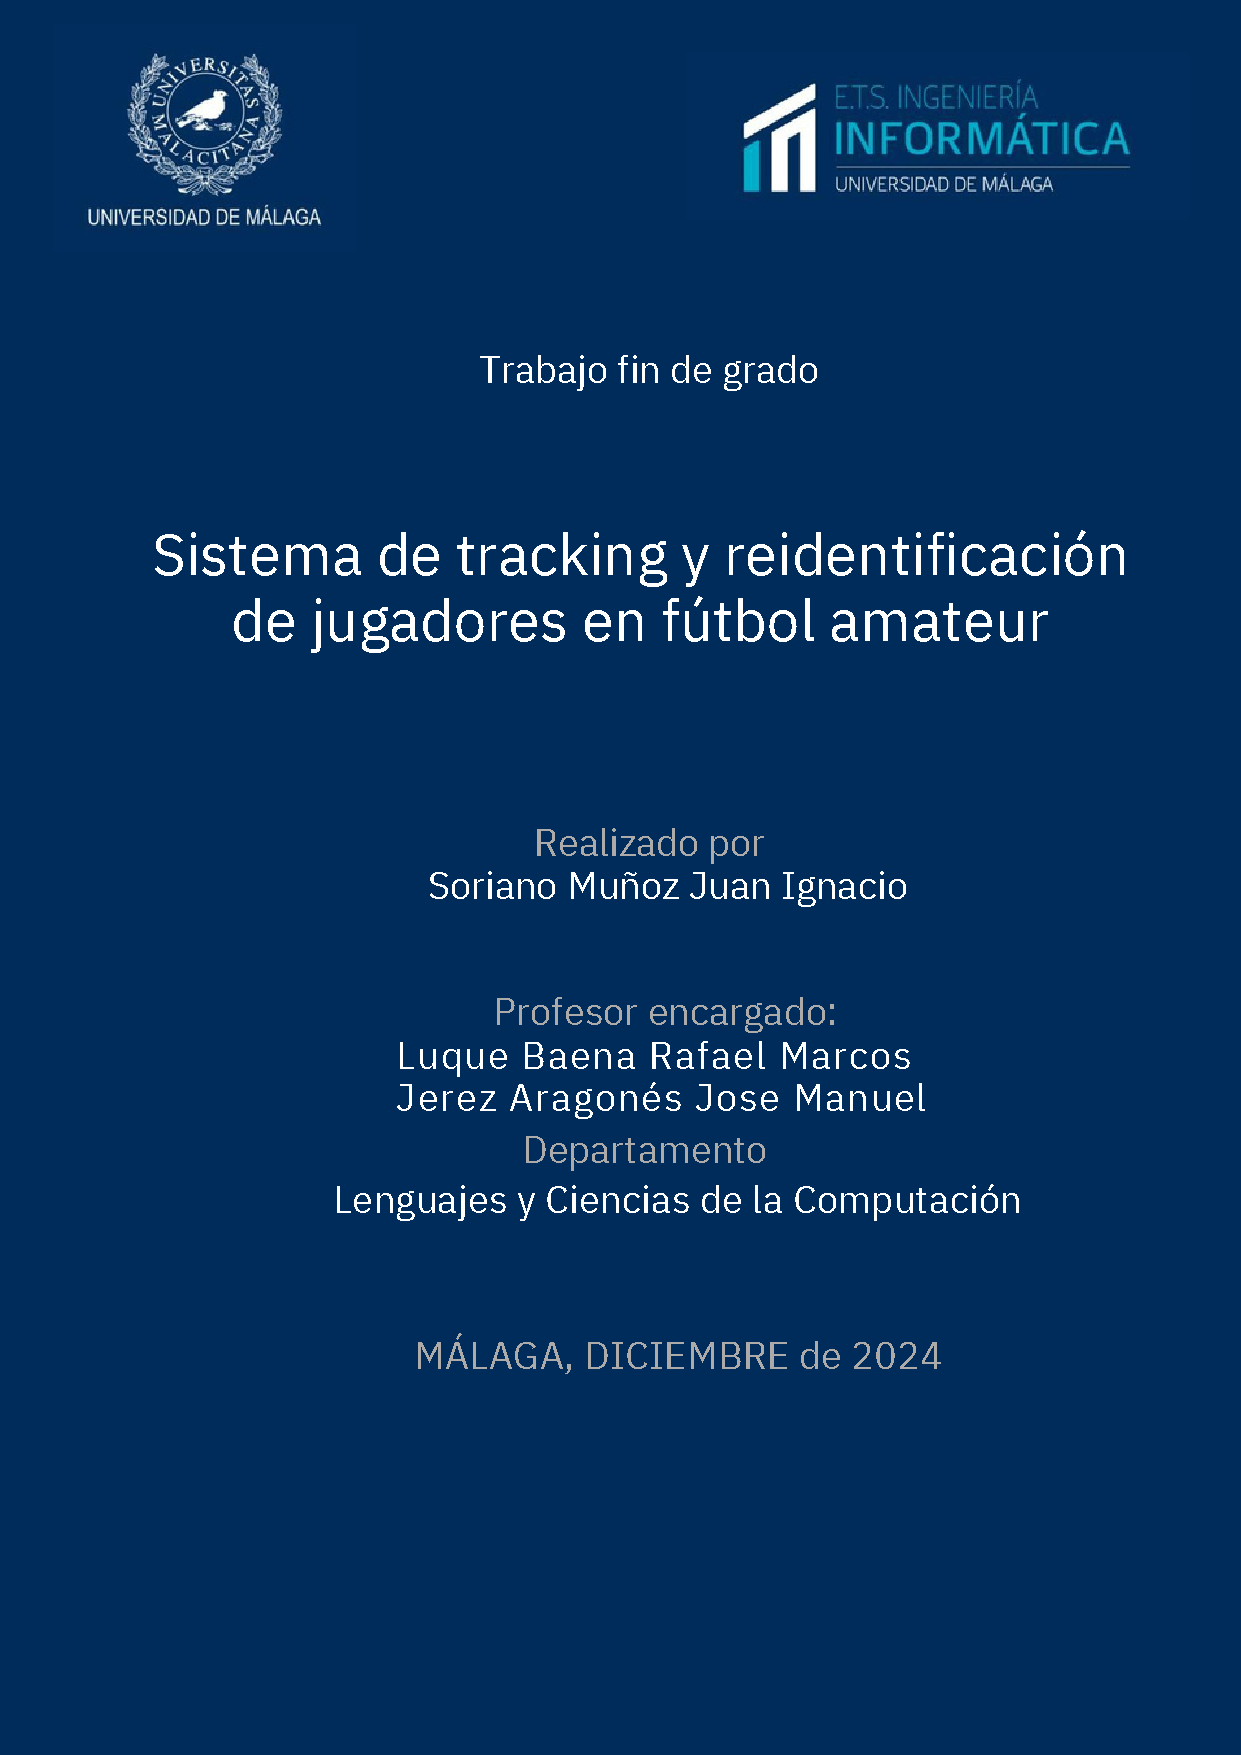
\includepdf[noautoscale=true, width=\paperwidth]{cover.pdf}
	
	%% Title
	\clearpage
	\setcounter{page}{1}
	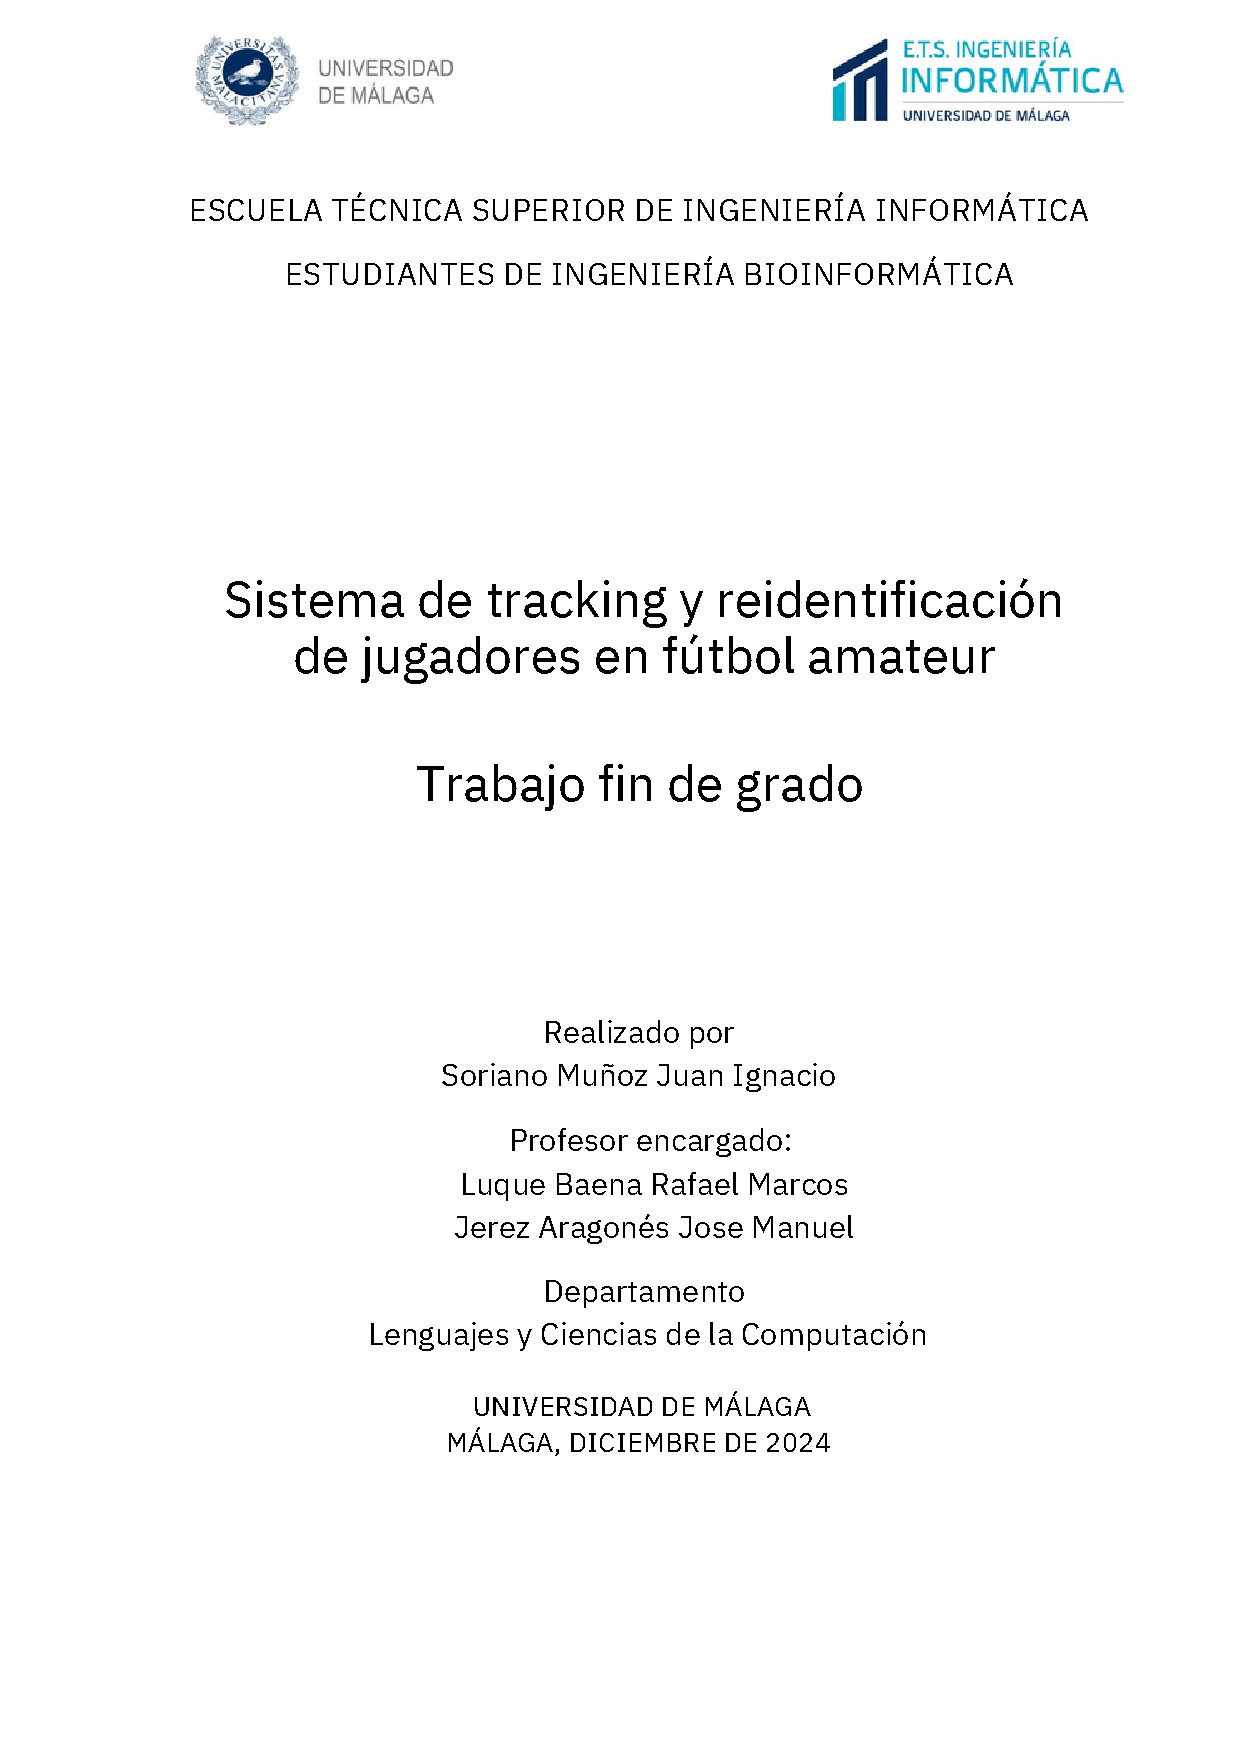
\includepdf[noautoscale=true, width=\paperwidth]{title.pdf}
	
	%%%%%%%%%%%%%%%%%%%%%%%%%%%%%%%%%%%%%%%%%%%%%%%%%%%%%%%%%%%%%%%%%%%%%%%%%%%
	
	% Índice automático
	\tableofcontents
	\newpage
	
	% Sections
	
		% Sections
	\section{Introducción}
	
	\section{Diario de avances}
	
	\subsection{Semana 3-16 de marzo)}
	
	Por ahora lo que llevamos es un dataset hecho en roboflow con un partido de España contra Suiza. Realizamos capturas y dividimos el conjunto en training, validation y test.
	
	Entrené el modelo de YOLO con este dataset revisado y el modelo no supo detectar bien el balón debido a la poca cantidad de imágenes donde se pueda ver bien la bola. El árbitro y los jugadores fueron bien detectados.
	
	Se replanteó el objetivo del TFG. Se focalizará en la reidentificación de jugadores cuando salen fuera de plano y en el desarrollo de una aplicación que permita al usuario decidir si cuando se produce un cambio de identificador, mantenerlo o cambiarlo, creando un dataset revisado.
	
	\subsection{Semana 17-31 de marzo \cite{sun2024gta}}
	
	A la hora de medir resultados como estas gráficas:
	
	\begin{figure}[h]
		\centering
		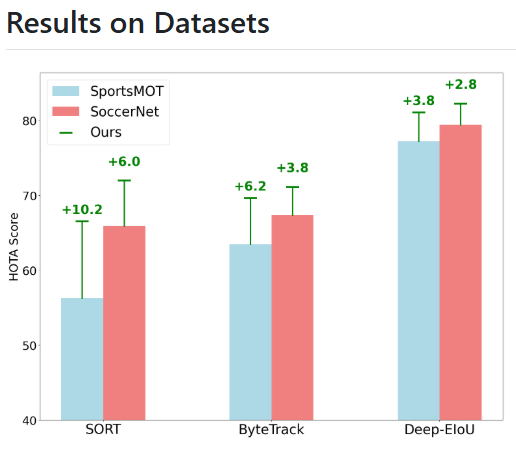
\includegraphics[width=0.8\textwidth]{image/metricasBeta}
		\caption{\textbf{Métricas gta\_link}}
		\label{fig:metricasBeta}
	\end{figure}
	
	Nos centraremos en la medida de los ID's intentando minimizarlos, lo máximo posible, ya que la métrica significa número de ids generados.
	
	\begin{figure}[h]
		\centering
		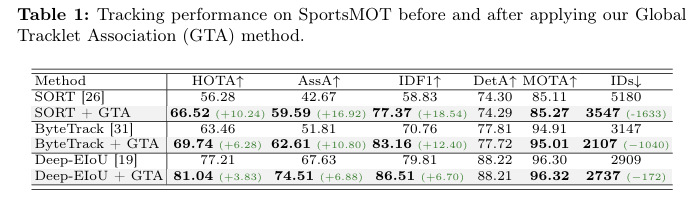
\includegraphics[width=0.8\textwidth]{image/Centrarse}
		\caption{\textbf{Objetivo}}
		\label{fig:Centrarse}
	\end{figure}
	
	Me he puesto a mirar lo que hace exactamente el código del repositorio de gta-link. Y en resumidas cuentas necesitamos un dataset con una pred, ya realizada, como es el caso de SoccerNet. Podemos descargar el dataset con el tracking realizado en los archivos .txt que se encuentran dentro de cada clip.\vspace{0.5cm}
	
	He utilizado las siguientes líneas de comando para realizar la descarga del dataset.
	
	\begin{verbatim}
		from SoccerNet.Downloader import SoccerNetDownloader
		mySoccerNetDownloader = SoccerNetDownloader(LocalDirectory="path/to/SoccerNet")
		mySoccerNetDownloader.downloadDataTask(task="tracking",
		 split=["train","test","challenge"])
	\end{verbatim}
	
	Posteriormente hice unos ajustes en el código para que cogiera los archivos \texttt{gt.txt} para que se tomara como referencia \textbf{--pred\_dir {tracking results directory}}, ya que estos son archivos \textbf{MOT}, que guardan información sobre los \textbf{bounding box} de cada objeto de cada frame, conteniendo información sobre \textbf{frame}, \textbf{id}, \textbf{bb\_left}, \textbf{bb\_top}, \textbf{bb\_width}, \textbf{bb\_height}, \textbf{conf}, \textbf{x}, \textbf{y}, \textbf{z}, en este orden.
	
	Estos son esenciales para que se pueda ejecutar el archivo \texttt{generate\_tracklets.py} para generar los \textbf{tracklets}.
	
	Un \textbf{tracklet} se genera al seguir a un objeto desde su detección en un fotograma hasta el siguiente. En este proceso, el código asocia las detecciones de objetos de cada fotograma con un identificador único (\textbf{ID}) para cada objeto, y los agrupa en una \textbf{"trayectoria"} que sigue ese objeto a lo largo del tiempo.
	
	En el código:
	
	\begin{itemize}
		\item \textbf{Extracción de características:} El código utiliza un modelo de reidentificación de personas (\texttt{FeatureExtractor}) para extraer características visuales de cada objeto detectado en los fotogramas. Esto es útil para seguir objetos entre fotogramas, incluso cuando se producen cambios de apariencia debido a variaciones en la vista o el movimiento.
		\item \textbf{Cálculo de tracklets:} Para cada fotograma, el código agrupa las detecciones de objetos utilizando el identificador único (\texttt{track\_id}). Si un objeto se detecta en un fotograma y luego aparece en otro, se agrega a un tracklet, que es una colección de todas las detecciones del mismo objeto a lo largo de varios fotogramas. Además, se guarda información como el puntaje de la detección y las características extraídas del modelo de reidentificación.
		\item \textbf{Salvado de tracklets:} Al final de cada secuencia de video o serie de fotogramas, los tracklets generados se guardan en un archivo \texttt{pickle} para su posterior uso, permitiendo analizar y trabajar con las trayectorias de los objetos en el futuro.
	\end{itemize}
	
	El programa \texttt{generate\_tracklets.py}, lo que hará será generar unos ficheros \texttt{.pkl} que guardan los datos de las trayectorias de los objetos detectados a lo largo del tiempo. Esto incluye, por ejemplo, las \textbf{detecciones de objetos en cada fotograma}, las \textbf{características extraídas por el modelo de reidentificación}, y los \textbf{identificadores únicos (ID)} asignados a cada objeto (en formato binario).
	
	Una vez que se tenga esos ficheros se realiza una \textbf{refinación de los tracklets} para evitar que se cambien los \textbf{ids con frecuencia}. Mejora los \textbf{tracklets} (trayectorias de objetos) generados por un \textbf{tracker en tareas de seguimiento de múltiples objetos (MOT)}. Utiliza dos componentes principales: el \textbf{Tracklet Splitter}, que divide \textbf{tracklets impuros} (con múltiples identidades) en subtracklets más precisos mediante \textbf{clustering (DBSCAN)}, y el \textbf{Tracklet Connector}, que fusiona \textbf{tracklets fragmentados} que pertenecen al mismo objeto basándose en \textbf{similitudes visuales y restricciones espaciales}. Los resultados refinados se guardan en archivos \texttt{.txt} en formato \textbf{MOT}, listos para su evaluación, visualización o análisis posterior. Este proceso optimiza la \textbf{precisión del seguimiento}, corrigiendo errores como \textbf{cambios de identidad} y \textbf{fragmentaciones}.\vspace{0.5cm}
	
	
	Ahora que tenemos un dataset etiquetado, tendremos que:
	
	\begin{itemize}
		\item \textbf{Encontrar una combinación de hiperparámetros óptima: } Con el objetivo de que el cambio de ids sea el mínimo posible.
		\item \textbf{Desarrollar una aplicación: } Con el objetivo de que avise al usuario sobre los cambios de id en los frames y confirme si está bien cambiado o debería conservarse el anterior.
	\end{itemize}
	
	\subsection{Semana 31-6 de abril)}
	
	En estas semanas hemos estado invirtiendo tiempo en las siguientes cosas. En un principio lo que teníamos era un dataset preparado con los ficheros ground truth fruto de un tracker usado (como DeepEIoU). Pero dado un vídeo, no podíamos aplicar los programas de gta-link, por lo que teníamos que conseguir los ficheros MOT de alguna manera. 
	
	Había dos opciones. La primera aplicar un tracker y la segunda aplicar un modelo de YOLO.
	
	Para la primera opción busqué en varios repositorios, que trataran con trackers, principalmente DeepEIoU, que es el tracker con el mejor rendimiento según las estadísticas de paperscode \cite{sportsmot_paperswithcode}.
	
	\begin{figure}[h]
		\centering
		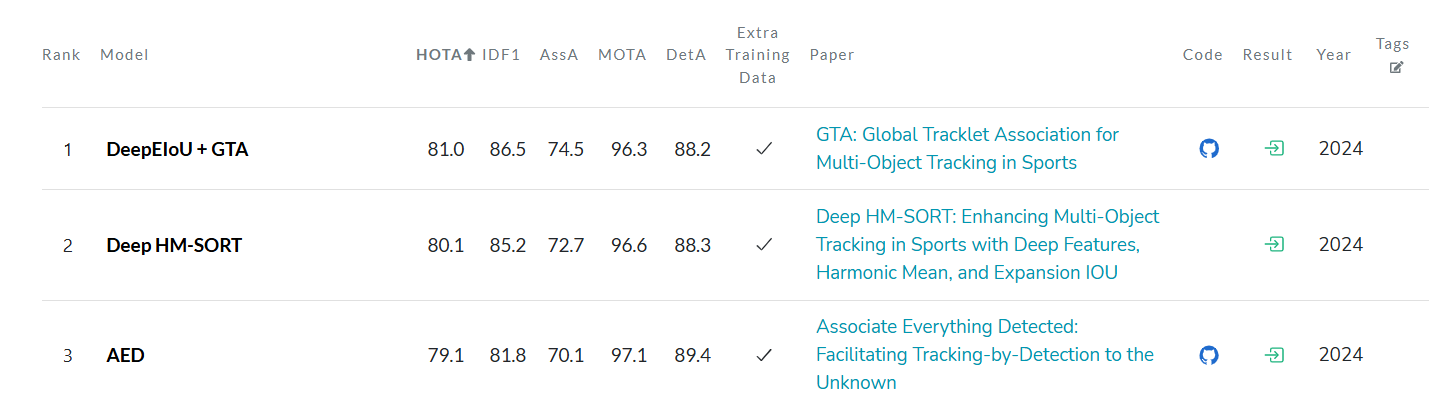
\includegraphics[width=0.8\textwidth]{image/deepEIoU}
		\caption{\textbf{Métricas DeepEIoU}}
		\label{fig:deepEIoU}
	\end{figure} 
	
	Tras encontrar un repositorio que trataba en específico con este \cite{huang2024iterative}. Tuve que modificar código para que utilizara cpu, ya que estaba configurado para gpu de nvidia. Los paquetes no se me instalaban correctamente. Los inputs que utilizaba para los programas eran ficheros tipo .npy.
	
	Dado que me estaba dando muchos problemas, después de dos días decidí que la mejor solución era utilizar un modelo de YOLO. Empecé utilizando un modelo de YOLO estandar capaz de detectar personas. El inconveniente de esto es que el video, estaba grabado desde un ángulo muy bajo, por lo que el modelo detectara las personas de las gradas y esto, a la larga, es un problema. 
	
	Entonces para resolver esto había dos opciones. La primera era realizar una segmentación del campo y la segunda entrenar un modelo de YOLO específico para jugadores. La segmentación del campo es demasiado costosa, porque no hay nada automatizado y sería segmentar infinidad de frames. Además de que es específica para un partido de fútbol en un ángulo en específico.Por lo tanto, la mejor opción para mi gusto es entrenar un modelo de YOLO con un dataset, por ahora, específico del partido de balonmano que me proporcionó mi tutor Jose Manuel Jerez. El dataset lo hice creando un programa utilizando las librerias de opencv (cv2) que extraía frames cada 20 segundos que transcurría de vídeo. Los 20 segundos previenen levemente más overfitting del que ocurre por tener frames del mismo partido. 
	
	Esta opción me permite etiquetar poco, ya que Roboflow tiene una herramienta de etiquetado automático una vez se han etiquetado unas cuantas imágenes, por lo que simplemente tuve que corregir aquellas imágenes con un mal etiquetado.
	
	Tras tener el dataset etiquetado le añadí algunas augmentations. 
	
	A la hora de entrenar el modelo lo hice con 25 epochs. Tardó hora y media en entrenarse.
	
	Apliqué los programas del repositorio de gta-link y los resultados del trackeo son muy buenos, pero la ReID no tiene nada que ver con los resultados tan consistentes del dataset de SoccerNet debido a que la grabación no es profesional.
	
	Aun así tras 23 intentos observe que los parámetros que daban mejores resultados eran los siguientes: --use\_split --min\_len 100 --eps 0.8 --min\_samples 10 --max\_k 4 --use\_connect --spatial\_factor 1.0 --merge\_dist\_thres 0.7   
	
	Recientemente le he añadido frames del partido de fútbol 7 al dataset de roboflow. Y he creado un nuevo modelo de YOLO entrenado exclusivamente con ese dataset.
	
	Los objetivos para la próxima semana:
	
	\begin{itemize}
		\item \textbf{Buscar como aplicar un tracker:} Después de aplicar un trackeo con YOLO, sería necesario aplicar DeepEIoU. Investigar si aplicar un doble gta-link puede funcionar para refinar los tracklets todavía más.
		\item \textbf{Seguir desarrollando la aplicación: } Con el objetivo de que avise al usuario sobre los cambios de id en los frames y confirme si está bien cambiado o debería conservarse el anterior. Ya tengo un programa prueba\_revision\_ReID.py, que funciona como prototipo, pero falta desarrollarlo mucho.
	\end{itemize}
	
	\subsection{Semana 7-13 de abril)}
	
	Al final el proceso de usar el tracker es obligatorio, ya que los objetos son detectados por YOLO, pero luego los ids son colocados por el tracker, y de ahí saldrán ficheros tipo MOT. Entonces tras aplicar YOLO para tener ficheros con la info de los bounding box sobre los jugadores intentaremos aplicarle un tracker y de ahí  un modelo de ReID, para posteriormente utilizar gta.
	
	Secuencia de trabajo: YOLO + DeepEIoU + GTA
	
	\subsection{Semana 7-13 de abril)}
	
	Planteé una estructura oficial de lo que llevo hecho para que sea más formal y dar contexto e información sobre todo lo que rodea las prácticas y el proyecto de TFG.
	
	\section{Motivación y Contexto}
	
	\subsection{¿Por qué es importante el análisis en fútbol amateur?}
	
	El análisis de rendimiento, la estadística avanzada y el seguimiento de jugadores han revolucionado el fútbol profesional. Sin embargo, en el fútbol amateur estas tecnologías todavía son muy poco accesibles.
	Poder aplicar técnicas de tracking y análisis en estos niveles permitiría:
	\begin{itemize}
		\item \textbf{Mejorar el entrenamiento de jugadores jóvenes.}
		\item \textbf{Facilitar la toma de decisiones a entrenadores y clubes pequeños.}
		\item \textbf{Promover el desarrollo del talento de forma más justa y basada en datos.}
	\end{itemize}
	
	\subsection{¿Qué problema hay actualmente?}
	
	La causa del primer problema que encontramos es la deficiencia en las infraestructuras tecnológicas para la práctica del fútbol amateur; el hecho de no disponer de sistemas avanzados que implementan las cámaras múltiples o los sensores del fútbol en el sector profesional, por el alto coste que implicaría el uso de las soluciones comerciales de tracking (GPS, cámaras VICON, sistemas ópticos, etc.) y la escasez de datos de movimiento y rendimiento que sufren las categorías base y amateur.
	
	\section{Objetivos}
	
	El presente proyecto tiene como principal objetivo colaborar en el análisis de los deportes a nivel de fútbol amateur implementando un sistema de detección automática, de seguimiento y de reidentificación de los jugadores. A día de hoy, existe una diferencia muy considerable entre la tecnología que existe para el análisis táctico y de rendimiento del fútbol profesional y la del ámbito amateur, lo cual significa que clubes, entrenadores y jugadores amateurs no tienen las herramientas disponible para realizar un análisis automatizado y estructurado de sus partidos.
	Este trabajo pretende eliminar esta desigualdad creando un flujo de trabajo modular y eficiente que permita aplicar tecnología avanzada de visión por computador en el ámbito amateur. Para ello se combinan modelos de detección de objetos (YOLOX) con algoritmos de seguimiento multiobjeto (DeepEIoU) y técnicas de reidentificación de personas (ReID) con el modelo OSNet, las cuales son reforzadas con un refinamiento posterior (GTA-Link) que mejora la calidad de las trayectorias generadas.
	
	Los objetivos específicos del proyecto son los siguientes:
	
	\begin{itemize}
		\item Desarrollar un sistema capaz de identificar y seguir automáticamente a los jugadores durante el transcurso de un partido de fútbol grabado en vídeo.
		\item Implementar un modelo de reidentificación que permita mantener la coherencia de los IDs incluso ante desapariciones temporales del jugador en la escena.
		\item Aplicar técnicas de post-procesamiento para corregir errores comunes en los tracklets generados, como fragmentación o mezcla de identidades.
		\item Facilitar la reutilización y escalabilidad del flujo de trabajo en otros entornos deportivos, fomentando así su adopción por parte de entidades del fútbol base o amateur.
		\item Probar y validar el sistema sobre secuencias reales de fútbol amateur, evaluando su rendimiento en condiciones no controladas.
	\end{itemize}

	
	\section{Estado del sector}
	
	El análisis de rendimiento en el fútbol ha experimentado una transformación significativa en las últimas décadas, impulsada por avances tecnológicos que permiten una recopilación y procesamiento de datos cada vez más precisos y en tiempo real. Sin embargo, existe una marcada diferencia entre las herramientas utilizadas en el ámbito profesional y las accesibles para equipos amateurs.
	
	\subsection{Soluciones en el Ámbito Profesional}
	
	En el fútbol profesional, sistemas como TRACAB se han consolidado como referentes en el seguimiento y análisis de jugadores. TRACAB es un sistema de seguimiento óptico que utiliza cámaras y algoritmos de visión por computadora para rastrear en tiempo real la posición de todos los jugadores y el balón en el campo. Este sistema ha sido implementado en ligas de élite como la Premier League, La Liga y la Bundesliga, y está certificado por la FIFA para programas de seguimiento electrónico de rendimiento (EPTS). "https://tracab.com/products/tracab-technologies/?utm\_source=chatgpt.com"
	
	\begin{figure}[H]
		\centering
		\begin{minipage}{0.45\textwidth} % Controla el ancho de la imagen
			\centering
			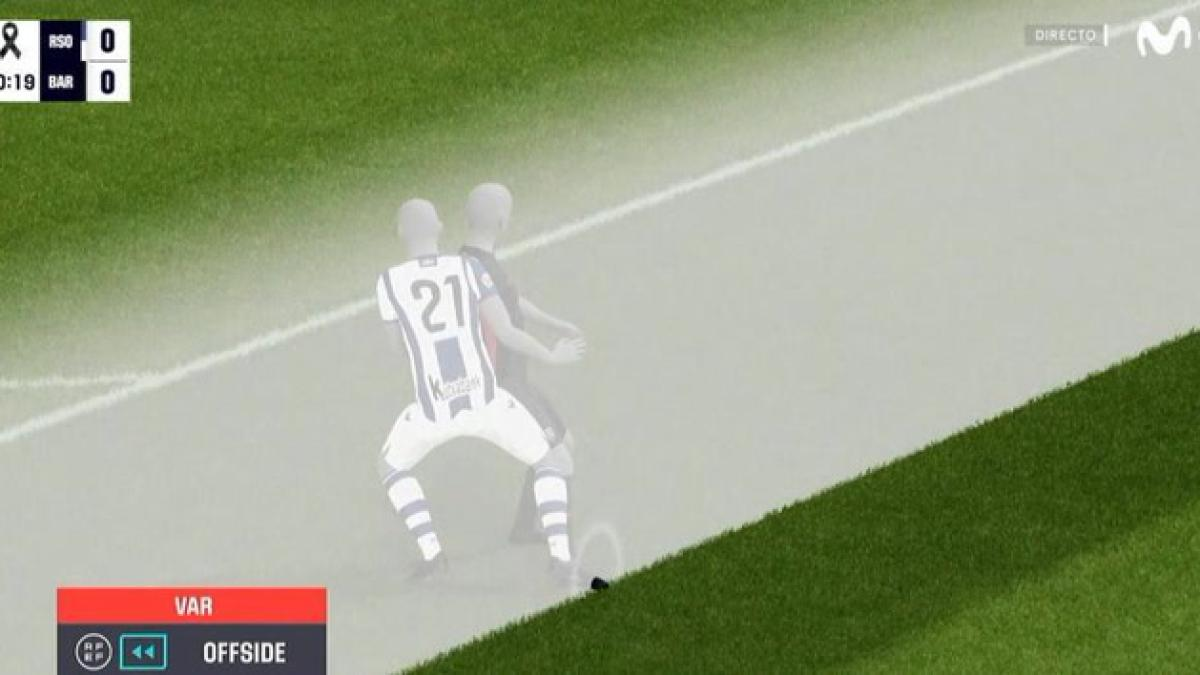
\includegraphics[width=\textwidth]{image/tracab}
			\label{tracab}
		\end{minipage}
		\hfill
		\begin{minipage}{0.45\textwidth} % Controla el ancho de la imagen
			\centering
			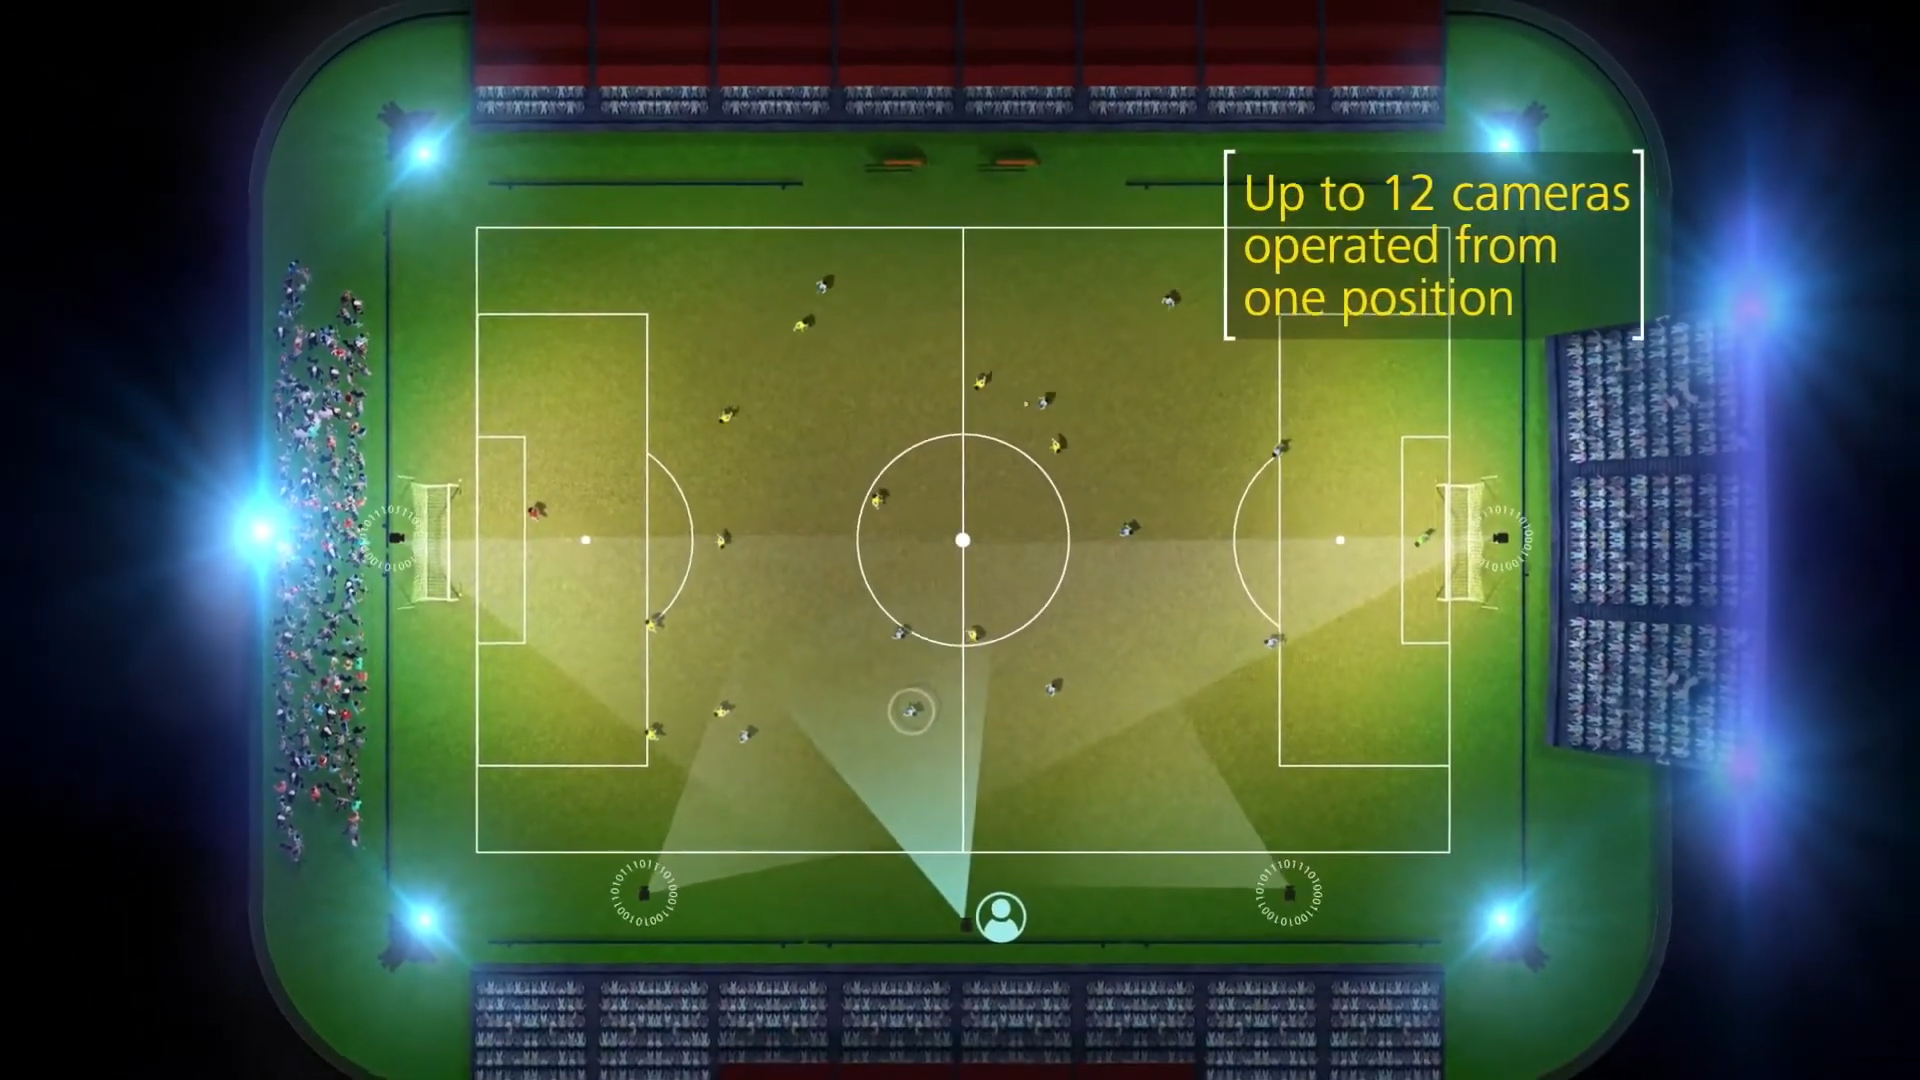
\includegraphics[width=\textwidth]{image/tracab2}
			\label{tracab2}
		\end{minipage}
		\caption{\textbf{Tracab}}
	\end{figure}
	
	
	\subsection{Herramientas Disponibles para el Fútbol Amateur}
	
	En contraste, el fútbol amateur ha comenzado a adoptar herramientas más asequibles y adaptadas a sus necesidades y recursos. Una de las más destacadas es LongoMatch, un software de análisis de vídeo que permite a entrenadores y analistas etiquetar eventos, crear estadísticas y generar informes tácticos a partir de grabaciones de partidos.
	
	\begin{figure}[h]
		\centering
		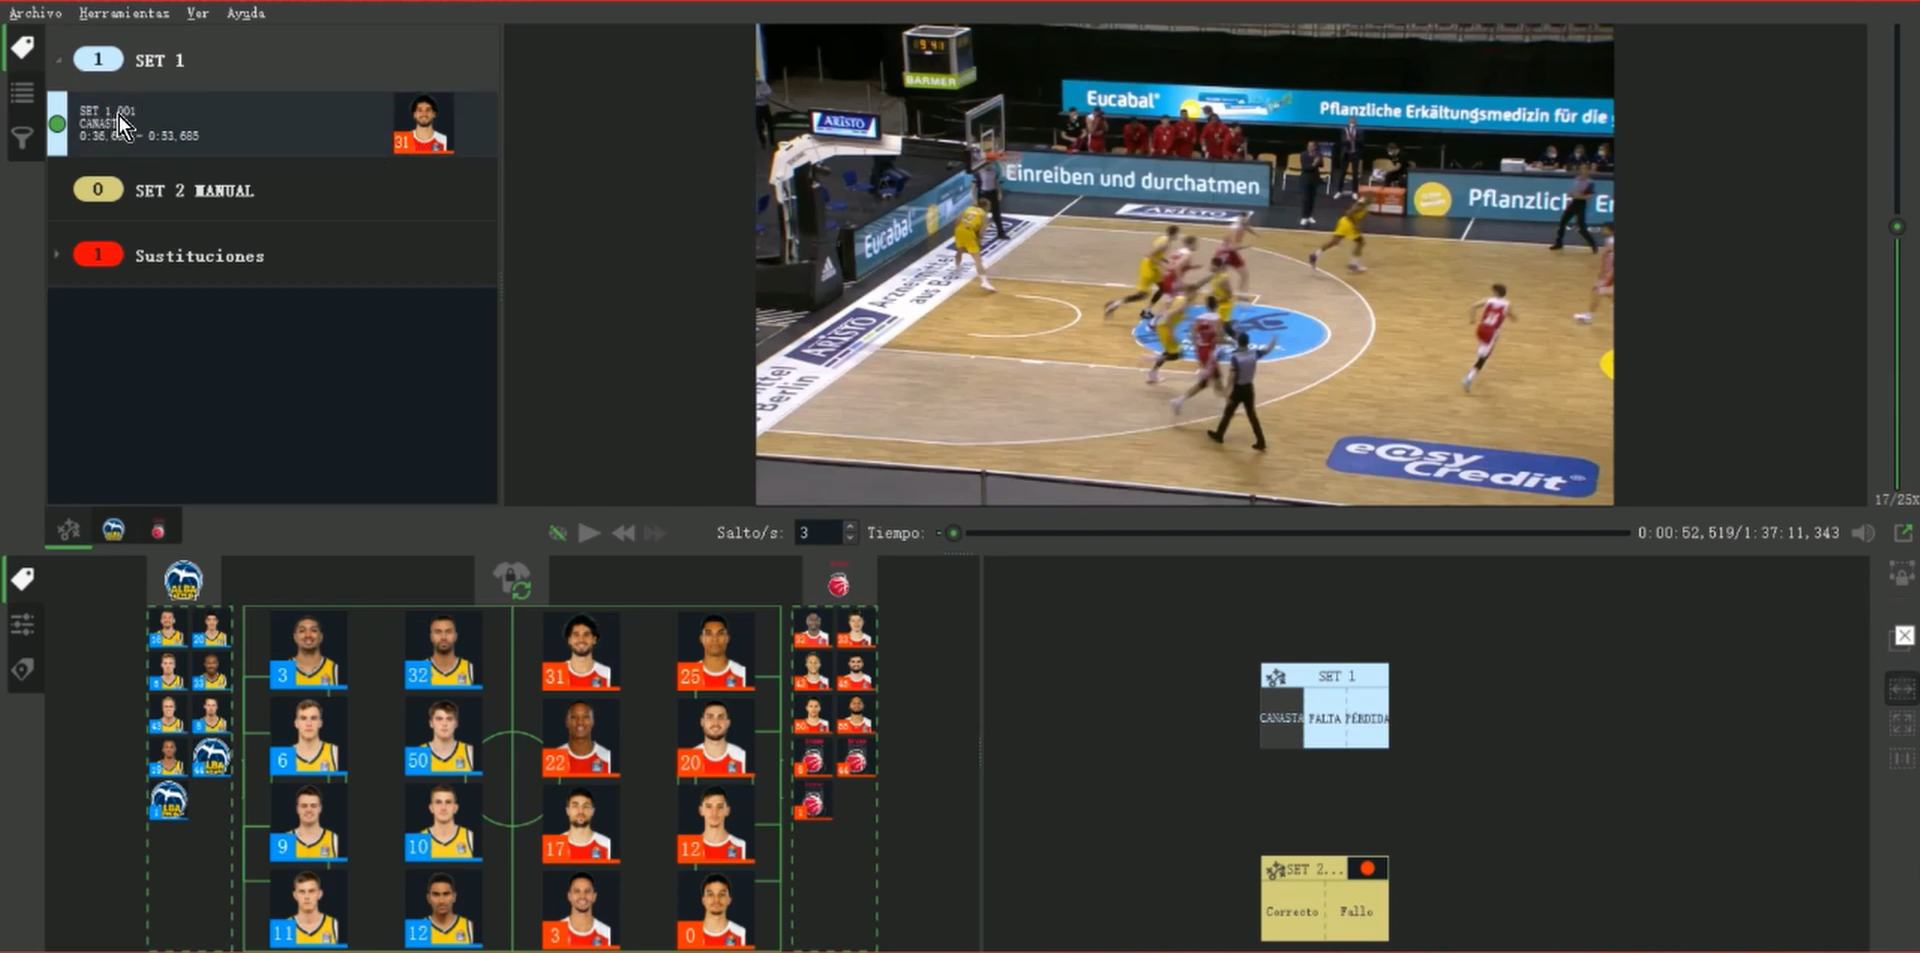
\includegraphics[width=0.8\textwidth]{image/longomatch}
		\caption{\textbf{Interfaz de Longomatch}}
		\label{fig:longomatch}
	\end{figure} 
	
	LongoMatch ofrece "https://longomatch.com/en/":
	\begin{itemize}
		\item	Análisis en tiempo real y post-partido con soporte para múltiples cámaras.

	
		\item Personalización de paneles de análisis según las necesidades del equipo.
	
		\item Exportación de datos y vídeos para compartir con jugadores y cuerpo técnico.
	
		\item Compatibilidad con diversas plataformas y dispositivos móviles.
	\end{itemize}
	
	Además, herramientas como PIX4TEAM 2 han emergido para automatizar la grabación de partidos sin necesidad de un operador de cámara, facilitando la recopilación de material para análisis en equipos con recursos limitados. "https://shop.movensee.com/es/content/31-pix4team-camara-automatica-para-los-deportes-colectivos"
	
	\subsection{Limitaciones}
	
	\begin{center}
		\begin{tabular}{|p{6.5cm}|p{6.5cm}|}
			\hline
			\textbf{Limitaciones del sector amateur} & \textbf{Aportaciones del presente proyecto} \\
			\hline
			Los sistemas comerciales como Second Spectrum o STATS SportVU requieren múltiples cámaras y hardware costoso. &
			Se utiliza vídeo monocámara accesible y fácil de capturar con dispositivos comunes. \\
			\hline
			Los trackers convencionales pierden frecuentemente la identidad del jugador en escenas con oclusiones o cambios de plano. &
			Se implementa un módulo de re-identificación (ReID) basado en TorchReID y OSNet para mantener la identidad a lo largo del partido. \\
			\hline
			No existen herramientas que generen anotaciones automáticas de forma sencilla a partir del vídeo. &
			Se desarrolla un flujo de trabajo que genera archivos de anotaciones (formato MOT) automáticamente a partir del vídeo de entrada. \\
			\hline
			Los modelos existentes están entrenados en entornos profesionales, con condiciones muy diferentes al fútbol amateur. &
			Los modelos utilizados en este proyecto han sido entrenados y validados específicamente sobre partidos de fútbol amateur. \\
			\hline
			Las soluciones actuales no están diseñadas para clubes pequeños: requieren licencias, suscripciones o personal técnico. &
			Se busca una solución reproducible, ligera y gratuita basada en herramientas \textit{open-source}, accesible a cualquier usuario técnico. \\
			\hline
		\end{tabular}
	\end{center}
	
	\section{Tecnologías empleadas}
	
	Este proyecto ha hecho uso de diversas tecnologías de software y frameworks de inteligencia artificial que permiten implementar un sistema de tracking con detección, seguimiento y reidentificación de jugadores en partidos de fútbol amateur. A continuación, se detallan las principales herramientas y recursos utilizados.
	
	\subsection{Programación}
	
	Para el desarrollo del sistema se ha utilizado el lenguaje de programación Python, por su gran ecosistema de librerías para visión por computadora y deep learning. El flujo de trabajo se ha dividido en diferentes etapas, desarrolladas principalmente en entornos Jupyter Notebook y scripts de Python:
	
	\begin{itemize}
		\item \textbf{Jupyter Notebook:} Se utilizó para entrenar el modelo de detección de objetos YOLO, aprovechando la facilidad para experimentar de forma interactiva con parámetros y visualizar resultados.
		\item \textbf{Python (scripts):} Fue empleado para el entrenamiento del modelo de re-identificación (ReID), así como para aplicar todos los modelos en el flujo final de inferencia y generación de vídeos etiquetados con las predicciones.
	\end{itemize}
	
	\subsection{Gestión de datos y flujo de trabajo}
	
	\textbf{Roboflow} ha sido una herramienta fundamental para gestionar el dataset de entrenamiento del detector YOLO. Roboflow permite subir imágenes, etiquetarlas, realizar aumentos de datos automáticamente y exportar el dataset en el formato deseado (en nuestro caso, YOLOv8).
	
	\textbf{GitHub} ha sido el sistema elegido para el control de versiones y colaboración. Se ha utilizado para organizar y almacenar los diferentes módulos del proyecto, así como mantener un historial ordenado de los avances y pruebas realizadas durante el desarrollo del TFG.
	
	\subsection{Modelos utilizados}
	
	\textbf{YOLO (You Only Look Once)} ha sido el modelo principal utilizado para la detección de jugadores. Su arquitectura permite realizar detección en tiempo real, con una alta precisión y bajo coste computacional. Se entrenó una versión ligera del modelo con imágenes de fútbol amateur obtenidas del dataset gestionado en Roboflow.
	
	\textbf{DeepEIoU} fue el algoritmo de tracking utilizado para asociar detecciones entre frames y mantener la identidad de cada jugador. DeepEIoU combina estrategias geométricas (IoU) y de apariencia (cuando se usa ReID), lo que mejora la robustez frente a oclusiones y cambios de plano.
	
	Este modelo ha sido clave para generar archivos de anotación con los ID temporales de los jugadores a lo largo del vídeo, y servir como base para el post-procesamiento posterior mediante GTA-Link.
	
	\textbf{TorchReID} se ha usado como framework para entrenar el modelo de re-identificación. Se utilizó el modelo \textit{osnet\_x1\_0}, que fue ajustado sobre imágenes recortadas de jugadores, organizadas en carpetas según su identidad. Este modelo se utilizó posteriormente para mejorar el seguimiento, reduciendo los cambios de identidad.
	
	
	
	\section{Módulo de detección (YOLO)}
	https://arxiv.org/abs/1506.02640
	
	\subsection{Arquitectura YOLO}
	
	YOLO (You Only Look Once) es una arquitectura de detección de objetos en imágenes y vídeos que ha destacado por su velocidad y precisión. La arquitectura original de YOLO, según la propuesta en el artículo de Redmon et al. (2016)\footnote{Redmon, J., Divvala, S., Girshick, R.,  Farhadi, A. (2016). You Only Look Once: Unified, Real-Time Object Detection. arXiv preprint arXiv:1506.02640.}, se inspira parcialmente en GoogleNet y está compuesta por 24 capas convolucionales, cuatro capas de agrupamiento máximo (max pooling) y dos capas totalmente conectadas al final.
	
	Antes de procesarse, la imagen de entrada es redimensionada a un tamaño fijo de 448x448 píxeles. El flujo interno de la red emplea convoluciones de tipo 1x1 que tienen como función principal reducir el número de canales de activación intermedios sin afectar a la información espacial. Posteriormente, se aplican convoluciones de 3x3 para capturar patrones locales más complejos. Cada una de estas capas es seguida por una función de activación ReLU, que introduce no linealidad al modelo, excepto en la capa de salida, donde se emplea una función de activación lineal.
	
	Además, para mejorar la estabilidad del entrenamiento y evitar el sobreajuste, se aplican técnicas como la normalización por lotes (Batch Normalization) y el abandono (Dropout). Estas estrategias permiten que el modelo generalice mejor ante nuevos datos y se mantenga robusto frente a variaciones del entorno.
	
	Esta arquitectura permite que YOLO realice detección de múltiples objetos en una sola pasada sobre la imagen (de ahí su nombre), lo que lo convierte en un modelo extremadamente eficiente para tareas en tiempo real.
	
	\subsection{¿Cómo funciona la detección de objetos con YOLO?}
	
	Una vez entendida la arquitectura interna de YOLO, es importante comprender cómo se lleva a cabo el proceso de detección de objetos. Para ello, se puede imaginar el caso práctico de una aplicación que detecta jugadores y balones de fútbol a partir de una imagen de vídeo.
	
	\begin{figure}[H]
		\centering
		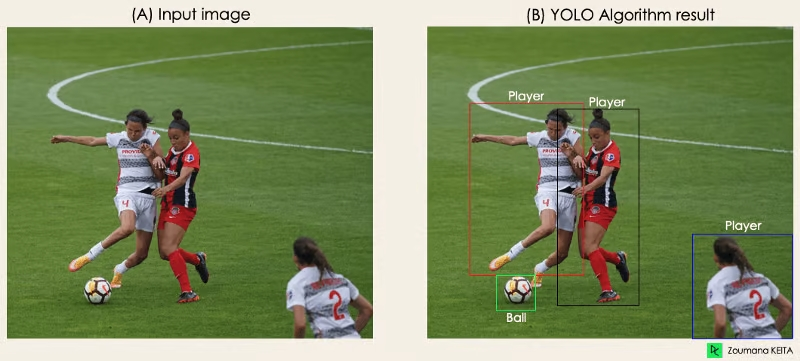
\includegraphics[width=0.8\textwidth]{image/yolodec1}
		\caption{\textbf{YOLO Detection. First Step}}
		\label{fig:YOLO Detection. First Step}
	\end{figure}
	
	El algoritmo de detección en YOLO se basa en cuatro pilares fundamentales: la división en cuadrículas, la regresión de cajas delimitadoras (bounding boxes), el cálculo del coeficiente de intersección sobre unión (IoU), y la supresión no máxima (NMS).
	
	\begin{enumerate}
		\item \textbf{División en cuadrículas (bloques residuales):} La imagen de entrada se divide en una cuadrícula de tamaño $N\times N$, donde cada celda es responsable de detectar los objetos que contiene. Cada celda predice una clase y una probabilidad asociada, además de parámetros que definen la caja delimitadora. 
		
		\begin{figure}[H]
			\centering
			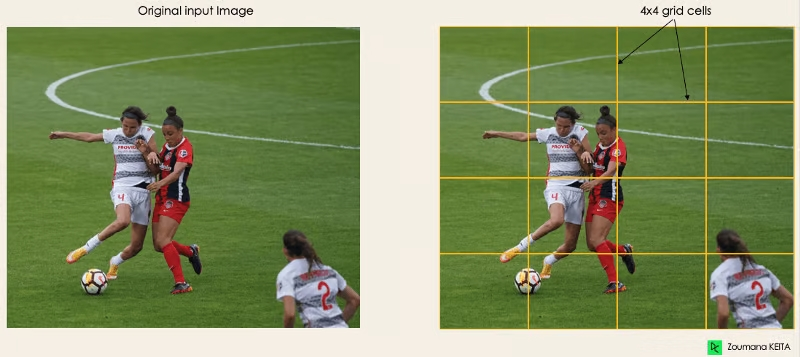
\includegraphics[width=0.8\textwidth]{image/yolodec2}
			\caption{\textbf{YOLO Detection. Second Step}}
			\label{fig:YOLO Detection. Second Step}
		\end{figure}
		
		
		\item \textbf{Regresión de cajas delimitadoras:} Cada celda predice varias cajas en el formato $Y = [p_c, b_x, b_y, b_h, b_w, c_1, c_2, \dots, c_n]$, donde:
		\begin{itemize}
			\item $p_c$ es la probabilidad de que la celda contenga un objeto.
			\begin{figure}[H]
				\centering
				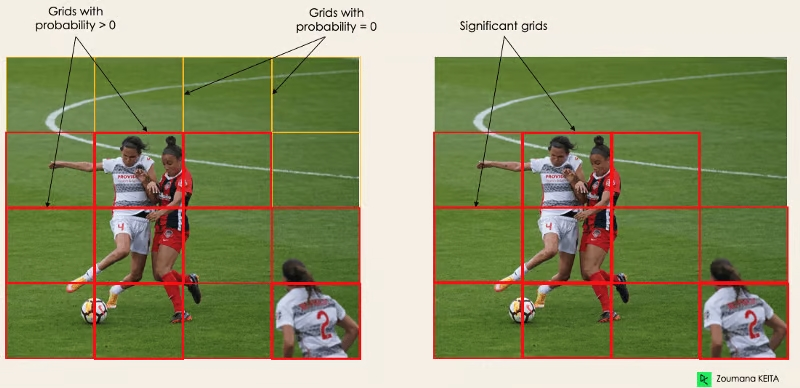
\includegraphics[width=0.8\textwidth]{image/yolodec3}
				\caption{\textbf{YOLO Detection. Third Step}}
				\label{fig:YOLO Detection. Third Step}
			\end{figure}
			\item $b_x$, $b_y$ son las coordenadas del centro de la caja respecto a la celda.
			\item $b_h$, $b_w$ son la altura y la anchura de la caja.
			\item $c_1, c_2, \dots$ son las probabilidades de pertenencia a cada clase (jugador, balón, etc.).
		\end{itemize}
		
		\begin{figure}[H]
			\centering
			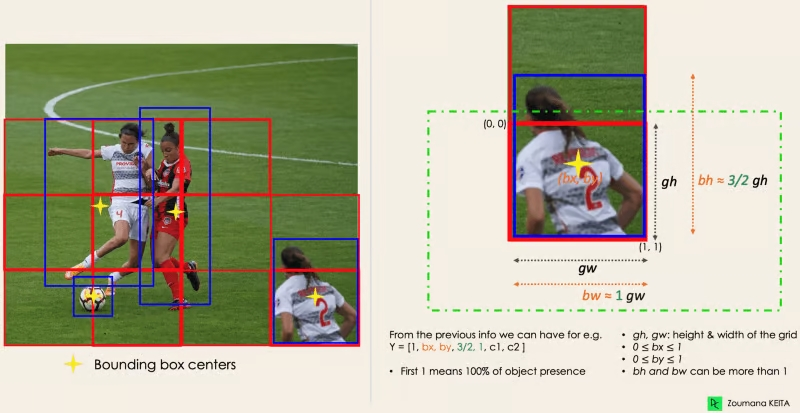
\includegraphics[width=0.8\textwidth]{image/yolodec4}
			\caption{\textbf{YOLO Detection. Fourth Step}}
			\label{fig:YOLO Detection. Fourth Step}
		\end{figure}
		
		
		
		
		\item \textbf{Intersección sobre Unión (IoU):} Para cada predicción, YOLO calcula el solapamiento entre la caja predicha y las cajas reales (ground truth). El valor del IoU (entre 0 y 1) permite descartar predicciones de baja calidad. Sólo aquellas con un IoU superior a un umbral son tenidas en cuenta.
		
		\begin{figure}[H]
			\centering
			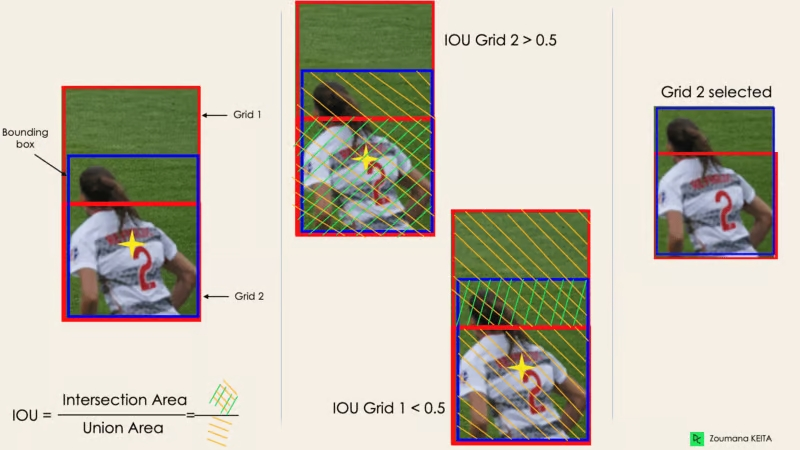
\includegraphics[width=0.8\textwidth]{image/yolodec5}
			\caption{\textbf{YOLO Detection. Fifth Step}}
			\label{fig:YOLO Detection. Fifth Step}
		\end{figure}
		
		
		\item \textbf{Supresión No Máxima (NMS):} Cuando varias cajas se solapan con valores altos de IoU, el algoritmo aplica NMS para conservar sólo la de mayor probabilidad, eliminando duplicados y reduciendo el ruido en las predicciones.
	\end{enumerate}
	
	Este proceso completo permite que, en un único paso y de forma muy eficiente, YOLO identifique múltiples objetos en una imagen, indicando su clase y ubicación precisa. Esta capacidad lo convierte en una herramienta especialmente útil en el análisis de vídeo deportivo, donde se requiere detectar varios jugadores en escenas rápidas y dinámicas.
	"https://www.datacamp.com/blog/yolo-object-detection-explained"
	
	
	\section{Módulo de tracking + Gestión de IDs}
	
	
	\subsection{Módulo de tracking}
	En el contexto de la detección de objetos en vídeo, como la realizada por modelos como YOLO, cada fotograma es procesado de forma independiente. Esto significa que, aunque el detector puede identificar y localizar objetos en cada imagen, no mantiene información sobre la identidad de estos objetos a lo largo del tiempo. Por ejemplo, no puede determinar si el jugador detectado en el fotograma 1 es el mismo que en el fotograma 2.
	
	Para abordar esta limitación, se emplean algoritmos de seguimiento de objetos (trackers) que asocian las detecciones entre fotogramas consecutivos, permitiendo así mantener la identidad de cada objeto a lo largo del tiempo. Estos trackers asignan un identificador único a cada objeto y actualizan su posición en cada nuevo fotograma, incluso en presencia de oclusiones o cambios de apariencia.
	
	\begin{figure}[H]
		\centering
		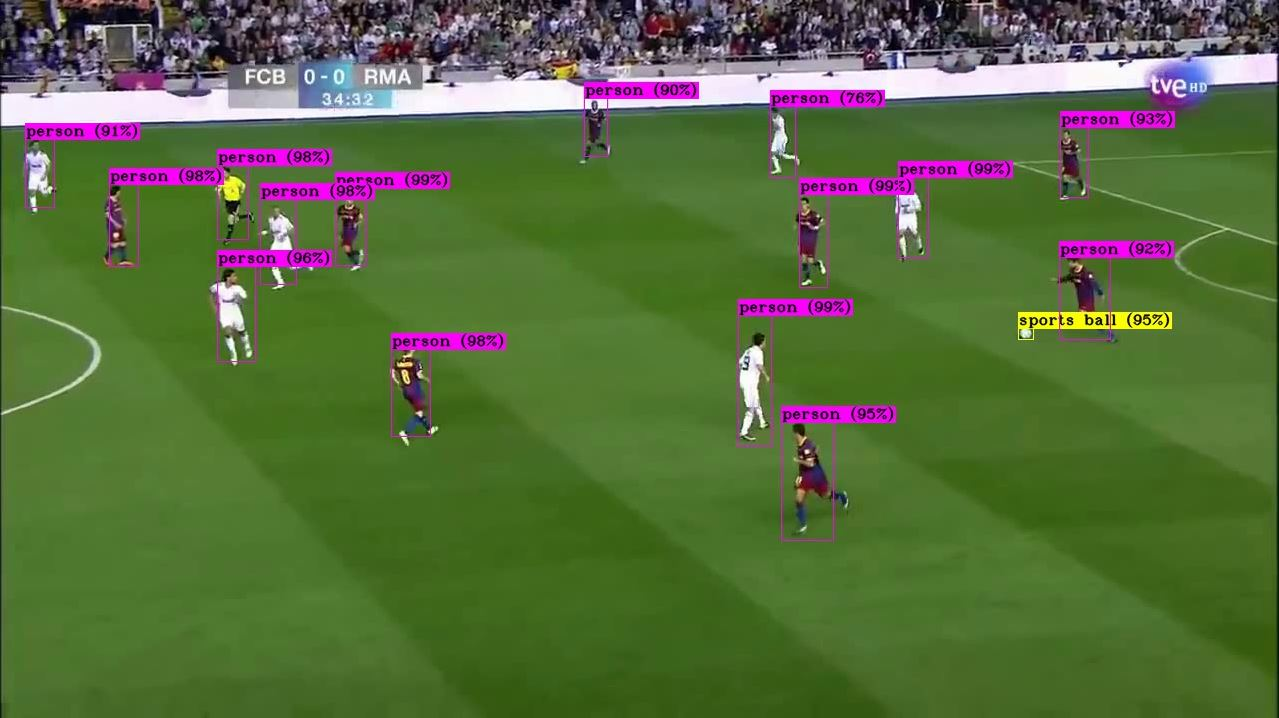
\includegraphics[width=0.8\textwidth]{image/tracking_id}
		\caption{\textbf{Tracking}}
		\label{tracking_id}
	\end{figure}
	
	Un ejemplo destacado de este enfoque es el algoritmo Deep SORT (Simple Online and Realtime Tracking with a Deep Association Metric), que combina información de movimiento y apariencia para asociar detecciones entre fotogramas. Deep SORT utiliza un filtro de Kalman para predecir la posición futura de los objetos y un descriptor de apariencia basado en redes neuronales profundas para comparar similitudes visuales entre detecciones. La asociación entre detecciones y trayectorias se realiza mediante el algoritmo húngaro, que minimiza el coste total de asociación considerando tanto la distancia de movimiento como la similitud de apariencia.
	"https://doi.org/10.1109/ICIP.2017.8296962"
	
	\subsection{Gestión de IDs}
	
	"https://paperswithcode.com/task/person-re-identification"
	
	La Re-identificación de Personas es una tarea de visión por computadora cuyo objetivo es asociar la identidad de una persona a través de diferentes cámaras o ubicaciones en una secuencia de vídeo o imágenes. Implica detectar y seguir a una persona y luego utilizar características como apariencia, forma del cuerpo y ropa para asociar su identidad en diferentes fotogramas. El objetivo es asociar a la misma persona en múltiples vistas de cámara no superpuestas de manera robusta y eficiente. 
	
	\begin{figure}[H]
		\centering
		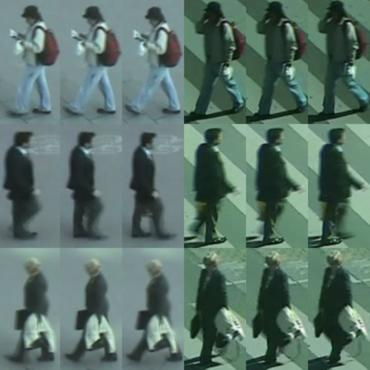
\includegraphics[width=0.4\textwidth]{image/gestion_id}
		\caption{\textbf{Person Re-Identification}}
		\label{gestion_id}
	\end{figure}
	
	
	\section{Propuesta}
	
	El flujo de trabajo propuesto tiene como objetivo optimizar el análisis de vídeos deportivos mediante un proceso de detección, seguimiento y reidentificación de jugadores, utilizando técnicas avanzadas de visión por computadora. El propósito es automatizar y mejorar la precisión en la identificación de jugadores a lo largo del vídeo, proporcionando un sistema que permita analizar el comportamiento de cada jugador durante el transcurso del partido.
	
	El resultado esperado de este flujo de trabajo es un archivo etiquetado que permita identificar a cada jugador con un seguimiento consistente a lo largo de las secuencias del video que utilizamos como input, lo que se traduce en un análisis más eficaz y exhaustivo. Este sistema facilitaría la recopilación de datos clave sobre el rendimiento individual de los jugadores, como su posición, movimientos y comportamientos durante el partido, ayudando a cerrar la brecha entre el análisis del fútbol profesional y el amateur.
	
	Al final del proceso, se espera obtener una salida en formato de vídeo con los jugadores anotados en el mismo y otra en formato MOT que contenga las trayectorias y las identificaciones de los jugadores, lo cual puede ser utilizado para estudios adicionales, análisis tácticos y optimización del rendimiento. Este flujo de trabajo proporciona la base para un sistema más completo y adaptable, capaz de integrarse con otras herramientas y métodos de análisis deportivos.
	
	\begin{figure}[H]
		\centering
		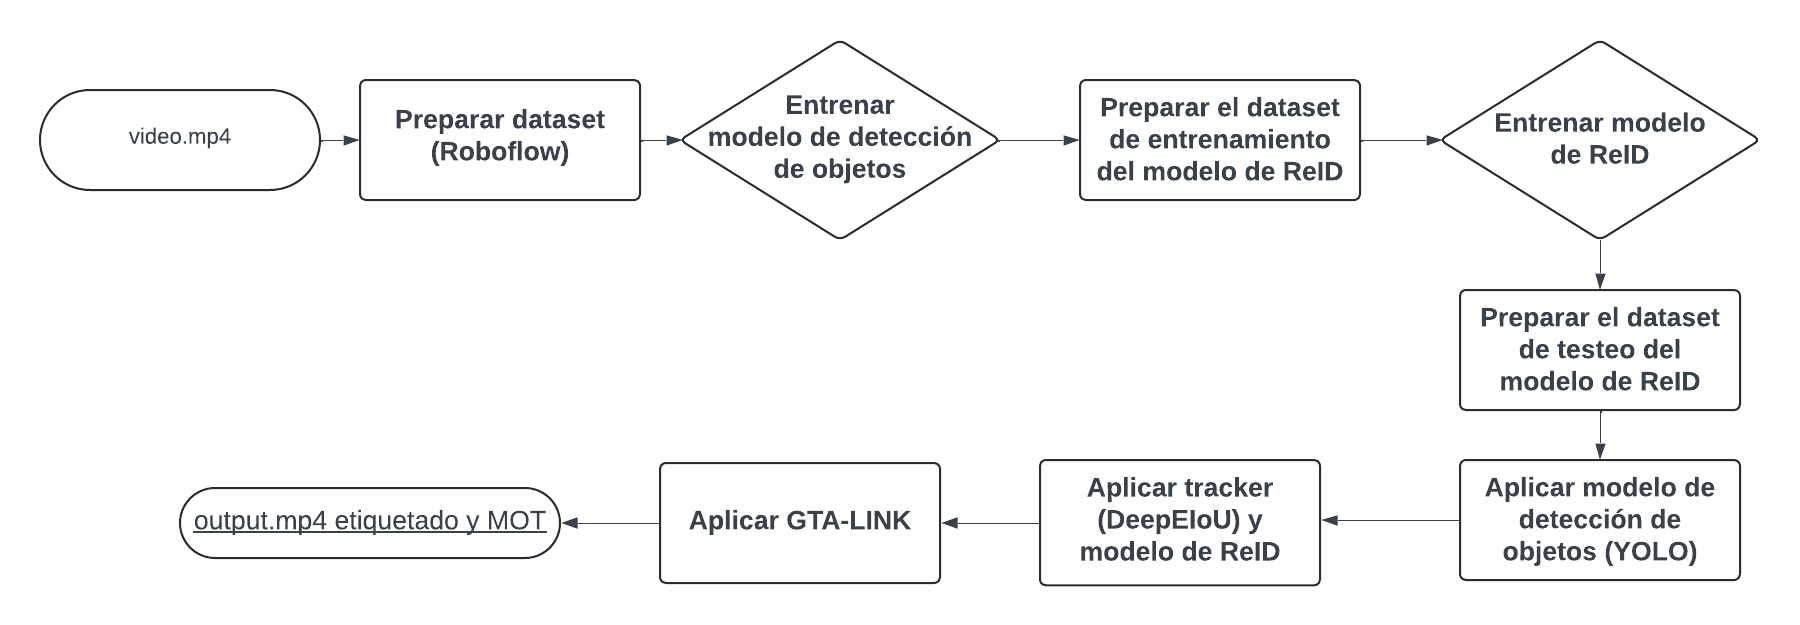
\includegraphics[width=0.8\textwidth]{image/Flowcharts}
		\caption{\textbf{Propuesta}}
		\label{fig:Propuesta}
	\end{figure}
	
	
	\section{Arquitectura general del sistema}
	
	A continuación, se explica paso a paso el flujo completo, desde la entrada de vídeo original hasta la salida final con el vídeo anotado y anotaciones generadas. Cada módulo del sistema se presenta de forma independiente, especificando su función dentro del flujo, la tecnología empleada y los beneficios que aporta al conjunto. \ref{fig:Propuesta}
	
	
	\subsection{Preparar el dataset (Roboflow)}
	
	https://roboflow.com/
	
	Para entrenar el modelo de detección de jugadores, utilizamos la plataforma Roboflow, una herramienta online ampliamente utilizada para gestionar datasets de visión por computador. Roboflow facilita la carga, etiquetado, preprocesado y exportación de conjuntos de datos en formatos compatibles con múltiples frameworks de deep learning, incluyendo YOLO.
	
	En nuestro caso, el proceso comenzó con la recopilación de fotogramas extraídos de vídeos de partidos de fútbol amateur. Estos frames fueron subidos a Roboflow, donde se realizó el etiquetado manual de los jugadores. Cada jugador fue anotado mediante la creación de una \textit{bounding box} alrededor de su figura, y se le asignó la clase \texttt{jugador}.
	
	Aunque en este proyecto únicamente se ha utilizado una clase (\texttt{jugador}), Roboflow permite una gestión flexible de múltiples clases. En el caso de que se hubiera querido incluir también la detección de otros roles como \texttt{árbitro} o \texttt{balón}, bastaría con asignar un nuevo nombre de clase a las anotaciones correspondientes durante el etiquetado. Cada vez que se etiqueta un objeto en un fotograma, se puede seleccionar (o crear) la clase deseada desde el menú desplegable de etiquetas.
	
	
	\begin{figure}[H]
		\centering
		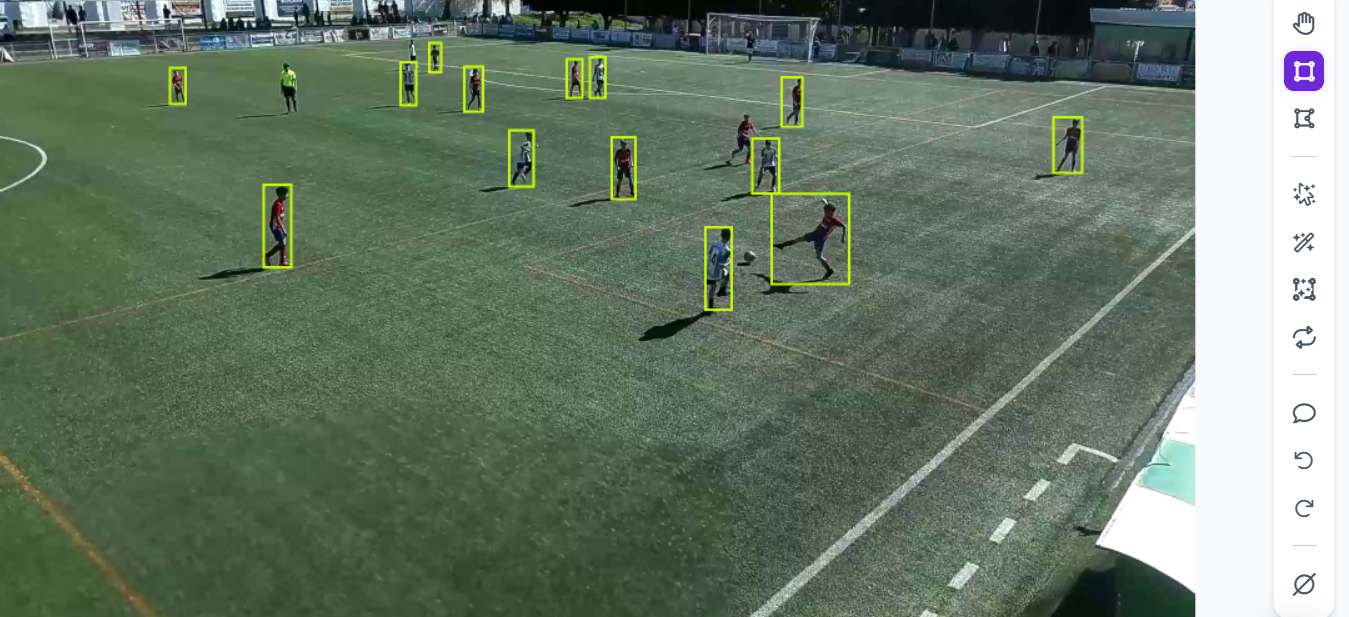
\includegraphics[width=0.8\textwidth]{image/dif_de_clases}
		\caption{\textbf{Diferenciación de clases}}
		\label{dif_de_clases}
	\end{figure}
	
	De este modo, el dataset resultante puede incluir múltiples clases, y el modelo YOLO aprenderá a diferenciarlas durante el entrenamiento, basándose en sus apariencias y posiciones relativas. Esta capacidad de distinguir entre diferentes tipos de objetos resulta esencial en contextos deportivos donde intervienen múltiples agentes.
	
	\begin{figure}[H]
		\centering
		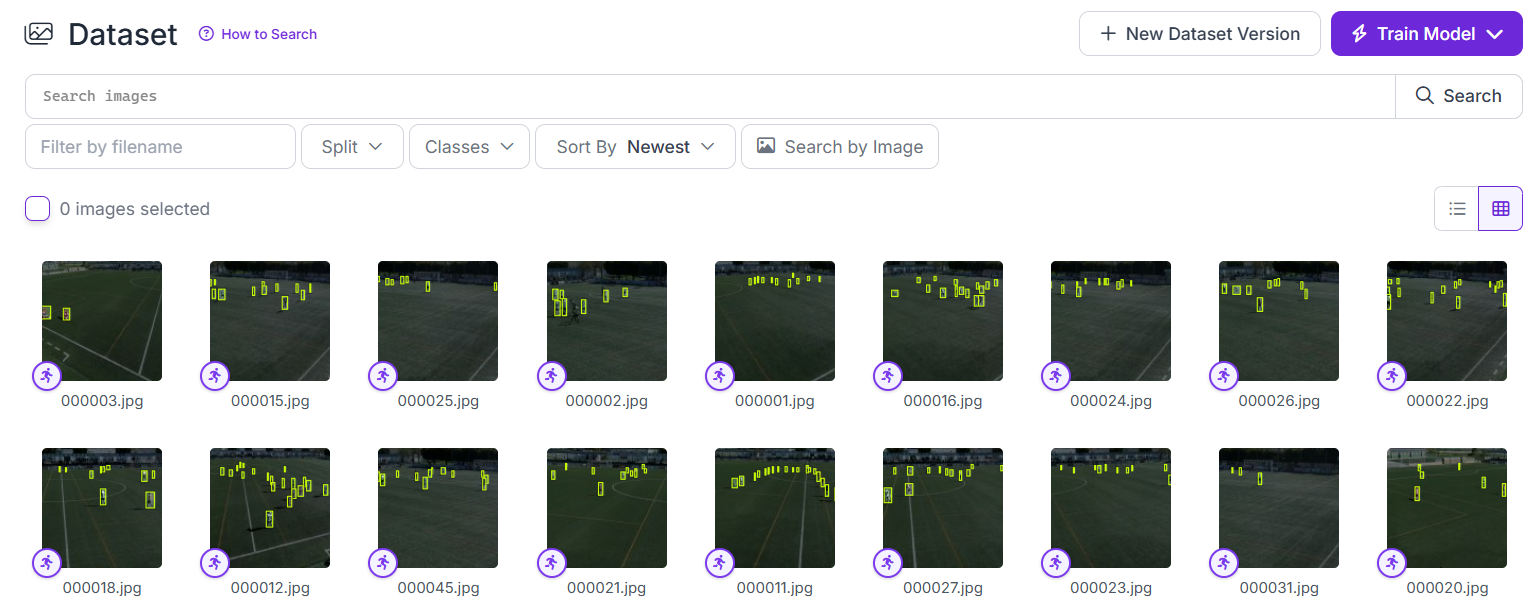
\includegraphics[width=0.8\textwidth]{image/entr_yolo}
		\caption{\textbf{Entrenamiento YOLO}}
		\label{entr_yolo}
	\end{figure}
	
	Una vez completado el etiquetado, el dataset fue exportado desde Roboflow en el formato YOLOv5/YOLOv8, incluyendo las anotaciones en archivos de texto por imagen, y un archivo \texttt{data.yaml} que especifica la configuración general del conjunto de datos, como las rutas, el número de clases y sus nombres.
	
	
	\subsection{Entrenamiento del modelo de YOLO}
	
	Una vez preparado el conjunto de datos en Roboflow y exportado en formato compatible con YOLOv8, se procedió al entrenamiento del modelo utilizando el framework \texttt{Ultralytics}, que proporciona una implementación optimizada y fácil de usar de los modelos YOLO.
	
	El entrenamiento se realizó en Python, comenzando por la descarga del dataset directamente desde la API de Roboflow. Para ello, se utilizó el siguiente fragmento de código:
	
	\begin{verbatim}
		from roboflow import Roboflow
		rf = Roboflow(api_key="sONwHlD0Zcp6DurtT8Nw")
		project = rf.workspace("pruebabalonmano").project("handball-dataset-def-2")
		version = project.version(1)
		dataset = version.download("yolov8")
	\end{verbatim}
	
	Este código descarga automáticamente las imágenes y las anotaciones en formato YOLOv8, incluyendo el archivo \texttt{data.yaml} con la configuración del dataset.
	
	A continuación, se cargó un modelo base preentrenado \texttt{yolov8n.pt} (versión ligera del modelo), y se inició el entrenamiento personalizado con los parámetros definidos:
	
	\begin{verbatim}
		from ultralytics import YOLO
		
		model = YOLO("yolov8n.pt")  # Modelo base preentrenado
		results = model.train(
		data=f"{dataset.location}/data.yaml",
		epochs=25,
		imgsz=640,
		batch=16,
		name="yolov8_handball"
		)
	\end{verbatim}
	
	En este caso, se entrenó durante 25 épocas, con imágenes de tamaño 640×640 píxeles y un tamaño de lote (\texttt{batch size}) de 16 imágenes. El modelo aprende a identificar la clase \texttt{jugador} a partir de los ejemplos anotados.
	
	Una vez finalizado el entrenamiento, se genera automáticamente el archivo \texttt{best.pt}, que contiene los pesos del modelo con mejor rendimiento en validación. Este modelo final puede utilizarse directamente para la inferencia:
	
	\begin{verbatim}
		best_model = YOLO("runs/detect/yolov8_handball/weights/best.pt")
	\end{verbatim}
	
	Este flujo de trabajo permite adaptar el modelo YOLOv8 a un dominio concreto, como el fútbol amateur, utilizando anotaciones específicas y obteniendo así un detector más ajustado al contexto real de aplicación.
	
	
	\subsection{Preparar el dataset de entrenamiento del modelo de ReID}
	
	El manejo de errores relacionados con la asignación incorrecta de IDs es un paso crucial en el proceso de reidentificación (ReID). Para resolver este problema, se utilizó un enfoque interactivo en el que se corrigen manualmente los errores de asignación de IDs en las anotaciones generadas por el modelo de ReID previamente entrenado con el dataset de SportMOT, que contiene imágenes de fútbol profesional.
	
	\subsubsection{annotate\_review.py}
	
	En primer lugar, las anotaciones de un partido de fútbol amateur fueron generadas utilizando el modelo de ReID entrenado con el dataset de SportMOT. Posteriormente, estas anotaciones fueron procesadas para corregir posibles errores de asignación de IDs. El código utilizado para este proceso interactivo es  y es el siguiente:
	
	\begin{verbatim}
		import os
		import cv2
		import argparse
		import tkinter as tk
		from tkinter import simpledialog
		from collections import Counter
		
		# Interactive MOT correction with flexible ID modification and distinct duplicate coloring
		
		def parse_mot_file(mot_path):
		entries = []
		with open(mot_path, 'r') as f:
		for line in f:
			if not line.strip(): continue
				parts = line.strip().split(',')
			entries.append({
				'frame': int(float(parts[0])), 
				'id': int(float(parts[1])), 
				'bbox': tuple(map(float, parts[2:6])),
				'raw': line.strip()
			})
		return entries
		
		
		def draw_annotations(img, detections, global_highlight=None, raw_color_map=None):
		out = img.copy()
		global_h = set(global_highlight or [])
		for det in detections:
			x, y, w, h = map(int, det['bbox'])
			tid = det['id']
			raw = det['raw']
			if raw_color_map and raw in raw_color_map:
				color = raw_color_map[raw]
			elif tid in global_h:
				color = (0, 0, 255)
			else:
				color = (0, 255, 0)
			cv2.rectangle(out, (x, y), (x + w, y + h), color, 2)
			cv2.putText(out, str(tid), (x, y - 5), cv2.FONT_HERSHEY_SIMPLEX, 0.5, color, 2)
		return out
	\end{verbatim}
	
	Este código permite corregir las asignaciones incorrectas de IDs mediante una interfaz gráfica que permite al usuario modificar o eliminar detecciones, asignar nuevos IDs a instancias específicas, y aprobar o eliminar duplicados.
	
	\textbf{Interacción del usuario:} La interacción con el programa es completamente visual e intuitiva. Al ejecutar el código, el usuario puede visualizar las detecciones en cada fotograma del video y recibir la opción de:
	
	\begin{itemize}
		\item Navegar entre los fotogramas (siguiente y anterior):
		\begin{lstlisting}[style=pythonstyle]
			if key == ord('n') and i < len(frames) - 1:
			i += 1
			elif key == ord('p') and i > 0:
			i -= 1
		\end{lstlisting}
		
		\item Modificar o eliminar instancias específicas de detecciones con IDs incorrectos:
		\begin{lstlisting}[style=pythonstyle]
			if key in (ord('m'), ord('d')):
			root = tk.Tk(); root.withdraw()
			prompt = "Introduzca 'i'<indice> para instancia o ID para global:"
			sel = simpledialog.askstring("Seleccionar deteccion", prompt)
			root.destroy()
			if not sel: continue
			if sel.startswith('i'):
			try:
			idx = int(sel[1:]) - 1
			chosen = duplicate_entries[idx]
			except:
			print("Seleccion invalida")
			continue
			if key == ord('m'):
			new_id = simpledialog.askinteger("Nuevo ID", "Nuevo ID para la instancia seleccionada:")
			if new_id is not None:
			raw_map[chosen['raw']] = new_id
			print(f"Instancia bbox {chosen['bbox']} mapeada a {new_id}")
			else:
			removed.add(chosen['raw'])
			print(f"Instancia bbox {chosen['bbox']} eliminada")
			else:
			try:
			orig = int(sel)
			except:
			print("ID invalido.")
			continue
			if key == ord('m'):
			new = simpledialog.askinteger("Nuevo ID", f"Nuevo ID para todas detecciones {orig}:")
			if new is not None:
			id_map[orig] = new
			print(f"Mapeado global ID {orig} -> {new}")
			else:
			for d in by_frame[orig_frame]:
			cur = raw_map.get(d['raw'], id_map.get(d['id'], d['id']))
			if cur == orig:
			removed.add(d['raw'])
			print(f"Todas detecciones ID {orig} eliminadas en frame {orig_frame}")
		\end{lstlisting}
		
		\item Corregir duplicados, donde se le presenta un mensaje con las IDs duplicadas detectadas en el fotograma:
		\begin{lstlisting}[style=pythonstyle]
			if duplicate_entries:
			dup_msgs = []
			dup_ids = []
			for idx_det, det in enumerate(duplicate_entries, 1):
			det_id = raw_map.get(det['raw'], id_map.get(det['id'], det['id']))
			name = color_names[(idx_det - 1) % len(color_names)]
			dup_msgs.append(f"{idx_det} ({name}) id {det_id}")
			dup_ids.append(det_id)
			print("Duplicados: " + ", ".join(dup_msgs) + f" en frame {orig_frame}")
		\end{lstlisting}
		
		\item Aceptar los cambios realizados y continuar con la corrección de otras detecciones:
		\begin{lstlisting}[style=pythonstyle]
			elif key == ord('c'):
			if duplicate_entries:
			approved_dup_ids.update(dup_ids)
			break
		\end{lstlisting}
	\end{itemize}
	
	
	El programa recorre automáticamente los fotogramas del video y, al detectar un nuevo ID, muestra una serie de opciones al usuario. Estos nuevos IDs se resaltan en rojo, lo que facilita su identificación como detecciones recién encontradas. Una vez que el usuario aprueba el ID, este se mantiene en verde, indicando que ha sido aprobado y no se volverá a revisar en el futuro. \ref{entr_reid}
	
	Este programa permite arreglar problemas graves de asignación de ids. Por ejemplo, que un jugador tenga un nuevo id durante el resto de la secuencia.
	
	\begin{figure}[H]
		\centering
		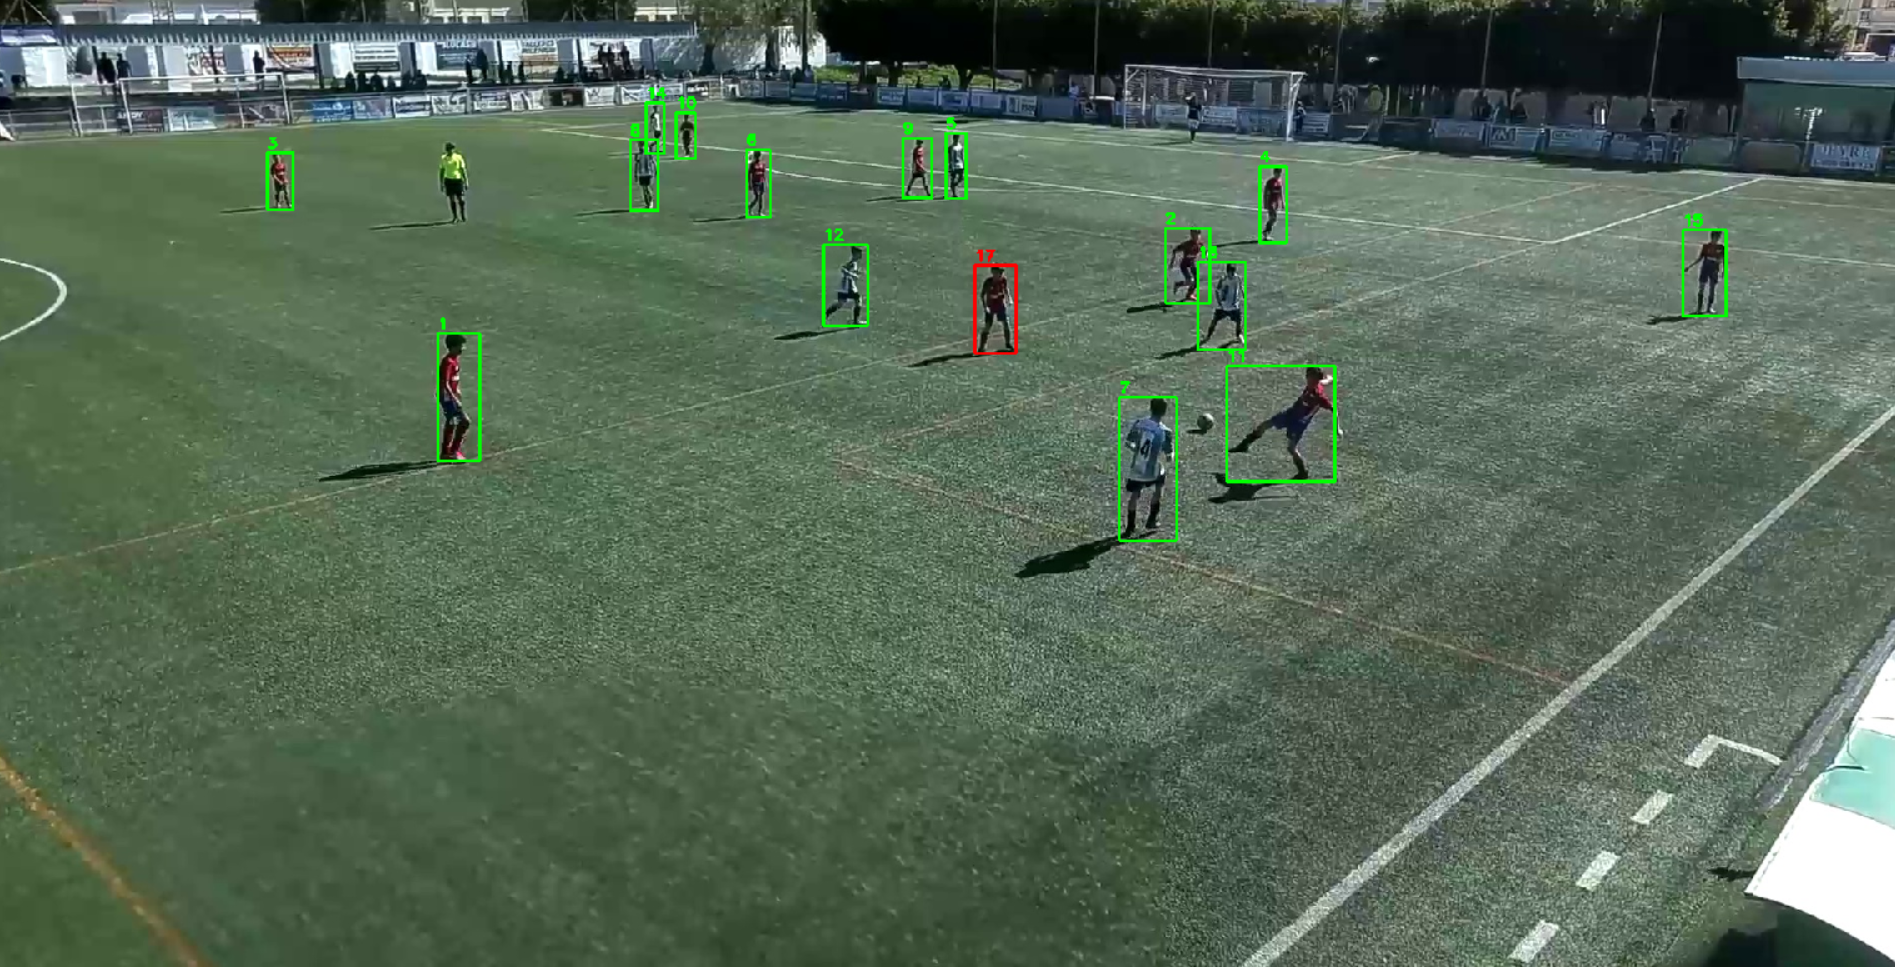
\includegraphics[width=0.8\textwidth]{image/entr_reid}
		\caption{\textbf{Programa para el entrenamiento}}
		\label{entr_reid}
	\end{figure}
	
	
	\subsubsection{annotate\_review\_precise.py}
	
	El programa \texttt{annotate\_review\_precise.py} es una versión complementaria del programa anterior \texttt{annotate\_review.py}.
	
	El código utilizado en este programa es el siguiente:
	\vspace{0.5cm}
	
	\begin{lstlisting}[style=pythonstyle]
		import os
		import cv2
		import argparse
		import tkinter as tk
		from tkinter import simpledialog
		from collections import Counter
		
		# Interactive MOT correction with manual frame control, per-frame ID modifications, approval colors, and undo
		
		def parse_mot_file(mot_path):
		entries = []
		with open(mot_path, 'r') as f:
		for line in f:
		if not line.strip(): continue
		parts = line.strip().split(',')
		entries.append({
			'frame': int(float(parts[0])),  # frame number
			'id':    int(float(parts[1])),  # original ID
			'bbox':  tuple(map(float, parts[2:6])),  # bbox
			'raw':   line.strip()  # raw line
		})
		return entries
		
		
		def draw_annotations(img, detections,
		new_ids, approved_new_ids,
		duplicate_entries, approved_dup_ids,
		raw_color_map=None, raw_index_map=None):
		out = img.copy()
		for det in detections:
		x, y, w, h = map(int, det['bbox'])
		tid = det['id']
		raw = det['raw']
		# determine color
		if raw_color_map and raw in raw_color_map:
		color = raw_color_map[raw]
		elif tid in approved_new_ids or tid in approved_dup_ids:
		color = (0, 255, 0)  # green approved
		elif tid in new_ids or any(d['id'] == tid for d in duplicate_entries):
		color = (0, 0, 255)  # red pending
		else:
		color = (0, 255, 0)
		# draw rectangle
		cv2.rectangle(out, (x, y), (x + w, y + h), color, 2)
		# prepare label
		label = str(tid)
		if raw_index_map and raw in raw_index_map:
		label += f"(i{raw_index_map[raw] + 1})"
		# put text
		cv2.putText(out, label, (x, y - 5), cv2.FONT_HERSHEY_SIMPLEX, 0.5, color, 2)
		return out
		
		
		def get_mapped_id(frame, det,
		id_map, raw_map,
		frame_id_map, frame_raw_map):
		# per-frame raw map
		if frame in frame_raw_map and det['raw'] in frame_raw_map[frame]:
		return frame_raw_map[frame][det['raw']]
		# per-frame id map
		if frame in frame_id_map and det['id'] in frame_id_map[frame]:
		return frame_id_map[frame][det['id']]
		# fallback global maps
		return raw_map.get(det['raw'], id_map.get(det['id'], det['id']))
		
		
		def pause_loop(by_frame, frames,
		id_map, raw_map,
		frame_id_map, frame_raw_map,
		removed, frames_dir,
		new_ids, duplicate_entries,
		approved_new_ids, approved_dup_ids,
		start_i):
		i = start_i
		orig_frame = frames[i]
		# color palette for duplicates
		palette = [(255, 0, 0), (255, 255, 0), (255, 0, 255), (0, 255, 255), (128, 0, 255)]
		raw_color_map = {d['raw']: palette[idx % len(palette)] for idx, d in enumerate(duplicate_entries)}
		raw_index_map = {d['raw']: idx for idx, d in enumerate(duplicate_entries)}
		
		# display duplicate info with indices
		if duplicate_entries:
		dup_info = ', '.join(f"i{idx+1}:{d['id']}" for idx, d in enumerate(duplicate_entries))
		print(f"Duplicados en frame {orig_frame}: {dup_info}")
		elif new_ids:
		print(f"Nuevos IDs en frame {orig_frame}: {new_ids}")
		print("Navegacion: [n]/[c]=next, [p]=prev, [u]=undo, [m]=modificar, [d]=delete, [q]=quit")
		
		while True:
		f2 = frames[i]
		dets2 = [d for d in by_frame[f2] if d['raw'] not in removed]
		mapped2 = []
		for d in dets2:
		mid = get_mapped_id(f2, d, id_map, raw_map, frame_id_map, frame_raw_map)
		mapped2.append({'bbox': d['bbox'], 'id': mid, 'raw': d['raw']})
		img2 = cv2.imread(os.path.join(frames_dir, f"{f2:06d}.jpg"))
		cv2.imshow('Annotations', draw_annotations(
		img2, mapped2,
		new_ids, approved_new_ids,
		duplicate_entries, approved_dup_ids,
		raw_color_map if f2 == orig_frame else None,
		raw_index_map if f2 == orig_frame else None
		))
		
		key = cv2.waitKey(0) & 0xFF
		if key in (ord('n'), ord('c')):
		approved_new_ids.update(new_ids)
		approved_dup_ids.update(d['id'] for d in duplicate_entries)
		return min(i + 1, len(frames) - 1), False
		elif key == ord('p'):
		return max(i - 1, 0), False
		elif key == ord('u'):
		return max(i - 1, 0), True
		elif key in (ord('m'), ord('d')):
		root = tk.Tk(); root.withdraw()
		sel = simpledialog.askstring("Seleccionar deteccion", "'i'<numero> o ID:")
		root.destroy()
		if not sel: continue
		# instance-level
		if sel.startswith('i'):
		try:
		idx = int(sel[1:]) - 1
		chosen = duplicate_entries[idx]
		except:
		print("Seleccion invalida"); continue
		if key == ord('m'):
		new_id = simpledialog.askinteger("Nuevo ID", "ID para esta instancia:")
		if new_id is not None:
		frame_raw_map.setdefault(orig_frame, {})[chosen['raw']] = new_id
		print(f"Instancia raw={chosen['raw']} -> {new_id} en frame {orig_frame}")
		else:
		removed.add(chosen['raw'])
		print("Instancia eliminada")
		# global-level
		else:
		try:
		orig = int(sel)
		except:
		print("ID invalido"); continue
		if key == ord('m'):
		new = simpledialog.askinteger("Nuevo ID", f"ID {orig} -> ? en frame {orig_frame}:")
		if new is not None:
		frame_id_map.setdefault(orig_frame, {})[orig] = new
		print(f"ID {orig} -> {new} en frame {orig_frame}")
		else:
		for d in by_frame[orig_frame]:
		cur = get_mapped_id(orig_frame, d, id_map, raw_map, frame_id_map, frame_raw_map)
		if cur == orig:
		removed.add(d['raw'])
		print(f"Instancias ID {orig} eliminadas en frame {orig_frame}")
		continue
		elif key == ord('q'):
		return len(frames), False
		else:
		continue
	\end{lstlisting}
	
	Este programa introduce varias mejoras y características adicionales respecto a la versión anterior:
	
	\begin{itemize}
		\item \textbf{Deshacer cambios:} La opción de deshacer (\texttt{[u]}) permite revertir los cambios realizados en el fotograma actual, añadiendo flexibilidad al proceso de corrección.
		\item \textbf{Visualización de duplicados mejorada:} Los duplicados se visualizan con colores específicos y se puede asignar un nuevo ID o eliminarlos en función de la decisión del usuario.
		\item \textbf{Control manual:} Se cambia la manera de recorrer los frames automáticamente a manualmente. Cada vez que se apruebe un frame se pasa al siguiente.
	\end{itemize}
	
	Este enfoque permite una corrección más precisa y segura, evitando acarrear ids erróneos.
	
	\begin{figure}[H]
		\centering
		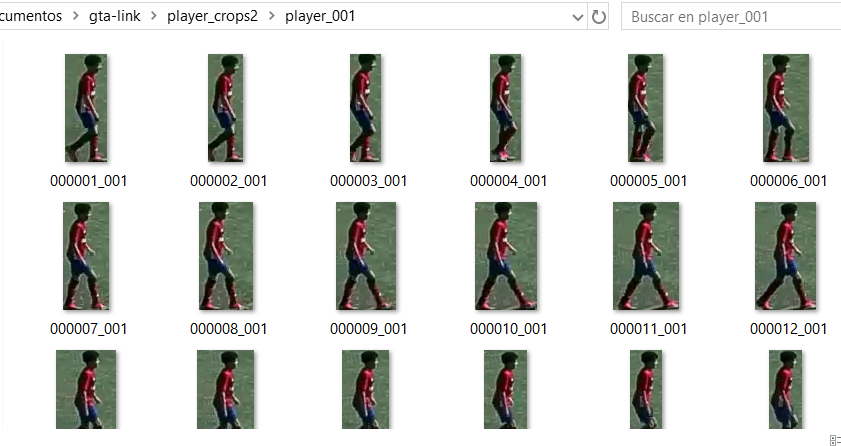
\includegraphics[width=0.8\textwidth]{image/dir_reid}
		\caption{\textbf{Estructura del dataset}}
		\label{dir_reid}
	\end{figure}
	
	\subsubsection{dicMaker\_idPlayer.py}
	
	El programa \texttt{dicMaker\_idPlayer.py} se utiliza para procesar un archivo MOT y generar recortes de imágenes de los jugadores en cada fotograma, organizados por ID de jugador. El archivo MOT contiene las anotaciones de las detecciones para cada fotograma, y el objetivo de este programa es generar recortes individuales de cada jugador basado en esas anotaciones.
	
	El proceso se realiza en dos etapas principales:
	
	1. \textbf{Lectura y análisis del archivo MOT:} El programa lee el archivo MOT que contiene las anotaciones de cada detección (frame, ID de jugador, coordenadas de la caja delimitadora) y organiza las detecciones por fotograma.
	
	2. \textbf{Recorte y guardado de las imágenes de los jugadores:} Para cada fotograma y cada jugador identificado en las detecciones, el programa recorta la región de la imagen correspondiente a las coordenadas de la caja delimitadora y guarda cada recorte en una carpeta organizada por ID de jugador.
	
	El código utilizado en este proceso es el siguiente:
	\vspace{0.5cm}
	
	\begin{lstlisting}[style=pythonstyle]
		import os 
		import cv2
		import argparse
		from tqdm import tqdm
		
		def parse_mot_file(mot_file_path):
		detections = {}
		with open(mot_file_path, 'r') as f:
		for line in f:
		parts = line.strip().split(',')
		if len(parts) < 6:
		continue
		
		frame_id = int(float(parts[0]))
		track_id = int(float(parts[1]))
		x, y, w, h = map(float, parts[2:6])
		
		if frame_id not in detections:
		detections[frame_id] = []
		detections[frame_id].append((track_id, int(x), int(y), int(w), int(h)))
		
		return detections
		
		def crop_and_save_detections(image_folder, detections, output_folder):
		os.makedirs(output_folder, exist_ok=True)
		
		for frame_id in tqdm(sorted(detections.keys()), desc="Procesando frames"):
		img_path = os.path.join(image_folder, f"{frame_id:06d}.jpg")
		
		if not os.path.exists(img_path):
		continue
		
		img = cv2.imread(img_path)
		if img is None:
		continue
		
		for track_id, x, y, w, h in detections[frame_id]:
		track_folder = os.path.join(output_folder, f"player_{track_id:03d}")
		os.makedirs(track_folder, exist_ok=True)
		
		x1 = max(0, x)
		y1 = max(0, y)
		x2 = min(img.shape[1], x + w)
		y2 = min(img.shape[0], y + h)
		
		if x2 <= x1 or y2 <= y1:
		continue
		
		crop = img[y1:y2, x1:x2]
		
		# Cambiado el nombre del archivo al formato deseado: frameId_trackId.jpg
		output_filename = f"{frame_id:06d}_{track_id:03d}.jpg"
		output_path = os.path.join(track_folder, output_filename)
		cv2.imwrite(output_path, crop)
		
		def main():
		parser = argparse.ArgumentParser()
		parser.add_argument('--mot_file', required=True)
		parser.add_argument('--image_folder', required=True)
		parser.add_argument('--output_folder', required=True)
		
		args = parser.parse_args()
		
		print("Leyendo archivo MOT...")
		detections = parse_mot_file(args.mot_file)
		
		print("\nRecortando detecciones...")
		crop_and_save_detections(args.image_folder, detections, args.output_folder)
		
		print(f"\nProceso completado. Recortes en: {args.output_folder}")
		
		if __name__ == "__main__":
		main()
	\end{lstlisting}
	\vspace{0.5cm}
	
	El programa realiza las siguientes funciones:
	
	\begin{itemize}
		\item \textbf{Parseo del archivo MOT:} El archivo MOT se procesa para organizar las detecciones por fotograma y por jugador. Cada detección incluye las coordenadas de la caja delimitadora y el ID de jugador.
		\item \textbf{Recorte de las imágenes:} Para cada fotograma y cada jugador detectado, se recorta la imagen según las coordenadas de la caja delimitadora. Los recortes se guardan en una estructura de carpetas donde cada jugador tiene su propia carpeta identificada por su \texttt{track\_id}.
		\item \textbf{Uso de la barra de progreso:} Se utiliza la librería \texttt{tqdm} para mostrar una barra de progreso durante el procesamiento de los fotogramas, facilitando el seguimiento del proceso.
	\end{itemize}
	
	
	\subsection{Entrenar el modelo de ReID}
	
	Para el entrenamiento del modelo de re-identificación (ReID), se utilizó el repositorio \texttt{Sportsreid}, que está basado en \texttt{SoccerNet Re-Identification} y \texttt{Torchreid}. Este repositorio permite reidentificar al mismo jugador en diferentes fotogramas de un video de un partido de fútbol. Sportsreid ha alcanzado el segundo puesto en el leaderboard de la división de prueba del reto SoccerNet 2022 de Re-Identification.
	
	El entrenamiento se lleva a cabo utilizando un archivo de configuración que define los parámetros del modelo, el optimizador y el scheduler, así como el conjunto de datos a utilizar. A continuación se describe el proceso de entrenamiento utilizando el archivo \texttt{main.py} proporcionado en el repositorio.
	
	El código de entrenamiento es el siguiente:
	\vspace{0.5cm}
	
	\begin{lstlisting}[style=pythonstyle]
		import sys
		import time
		import os.path as osp
		import argparse
		import torch
		import torch.nn as nn
		
		import torchreid
		from torchreid.reid.utils import (
		Logger, check_isfile, set_random_seed, collect_env_info,
		resume_from_checkpoint, load_pretrained_weights, compute_model_complexity
		)
		from default_config import (
		imagedata_kwargs, optimizer_kwargs, videodata_kwargs, engine_run_kwargs,
		get_default_config, lr_scheduler_kwargs
		)
		
		def build_datamanager(cfg):
		# ImageDataManager con batch sizes de train/test y relabel de IDs
		return torchreid.data.ImageDataManager(
		root=cfg.data.root,
		sources=tuple(cfg.data.sources),
		targets=(),                          # sin target set separado
		height=cfg.data.height,
		width=cfg.data.width,
		batch_size_train=cfg.train.batch_size,
		batch_size_test=cfg.test.batch_size,
		transform_train=cfg.data.transforms,
		transform_test=cfg.data.transforms,
		combineall=cfg.data.combineall,
		relabel=True,                        # remapea IDs a [0..N-1]
		num_workers=cfg.data.workers,
		verbose=True,
		use_gpu=cfg.use_gpu
		)
		
		def build_engine(cfg, datamanager, model, optimizer, scheduler):
		if cfg.data.type == 'image':
		if cfg.loss.name == 'softmax':
		engine = torchreid.engine.ImageSoftmaxEngine(
		datamanager,
		model,
		optimizer=optimizer,
		scheduler=scheduler,
		use_gpu=cfg.use_gpu,
		label_smooth=cfg.loss.softmax.label_smooth
		)
		else:
		engine = torchreid.engine.ImageTripletEngine(
		datamanager,
		model,
		optimizer=optimizer,
		margin=cfg.loss.triplet.margin,
		weight_t=cfg.loss.triplet.weight_t,
		weight_x=cfg.loss.triplet.weight_x,
		weight_tc=cfg.loss.triplet.weight_tc,
		weight_cc=cfg.loss.triplet.weight_cc,
		scheduler=scheduler,
		use_gpu=cfg.use_gpu,
		label_smooth=cfg.loss.softmax.label_smooth,
		topk=cfg.loss.triplet.topk,
		bottomk=cfg.loss.triplet.bottomk,
		warmup_lr=cfg.train.warmup_lr,
		warmup_steps=cfg.train.warmup_steps,
		lr=cfg.train.lr
		)
		else:
		if cfg.loss.name == 'softmax':
		engine = torchreid.engine.VideoSoftmaxEngine(
		datamanager,
		model,
		optimizer=optimizer,
		scheduler=scheduler,
		use_gpu=cfg.use_gpu,
		label_smooth=cfg.loss.softmax.label_smooth,
		pooling_method=cfg.video.pooling_method
		)
		else:
		engine = torchreid.engine.VideoTripletEngine(
		datamanager,
		model,
		optimizer=optimizer,
		margin=cfg.loss.triplet.margin,
		weight_t=cfg.loss.triplet.weight_t,
		weight_x=cfg.loss.triplet.weight_x,
		scheduler=scheduler,
		use_gpu=cfg.use_gpu,
		label_smooth=cfg.loss.softmax.label_smooth
		)
		return engine
		
		def reset_config(cfg, args):
		# Ruta por defecto a tu carpeta GTA-Link
		cfg.data.root = args.root or r'C:\Users\jismbs\Documents\gta-link'
		# Dataset de entrada por defecto
		cfg.data.sources = args.sources or ['player_crops2']
		# Transforms si se especifican
		if args.transforms:
		cfg.data.transforms = args.transforms
		
		def check_cfg(cfg):
		if cfg.loss.name == 'triplet' and cfg.loss.triplet.weight_x == 0:
		assert cfg.train.fixbase_epoch == 0, \
		'The output of classifier is not included in the computational graph'
		
		def main():
		parser = argparse.ArgumentParser(
		formatter_class=argparse.ArgumentDefaultsHelpFormatter
		)
		parser.add_argument(
		'--config-file', type=str, default='', help='path to config file'
		)
		parser.add_argument(
		'-s', '--sources', type=str, nargs='+',
		help='source datasets (delimited by space)'
		)
		parser.add_argument(
		'-t', '--targets', type=str, nargs='+',
		help='target datasets (delimited by space)'
		)
		parser.add_argument(
		'--transforms', type=str, nargs='+', help='data augmentation'
		)
		parser.add_argument(
		'--root', type=str, default='', help='path to data root'
		)
		parser.add_argument(
		'opts', default=None, nargs=argparse.REMAINDER,
		help='Modify config options using the command-line'
		)
		args = parser.parse_args()
		
		cfg = get_default_config()
		cfg.use_gpu = torch.cuda.is_available()
		if args.config_file:
		cfg.merge_from_file(args.config_file)
		reset_config(cfg, args)
		cfg.merge_from_list(args.opts)
		set_random_seed(cfg.train.seed)
		check_cfg(cfg)
		
		log_name = 'test.log' if cfg.test.evaluate else 'train.log'
		log_name += time.strftime('-%Y-%m-%d-%H-%M-%S')
		sys.stdout = Logger(osp.join(cfg.data.save_dir, log_name))
		
		print('Show configuration\n{}\n'.format(cfg))
		print('Collecting env info ...')
		print('** System info **\n{}\n'.format(collect_env_info()))
		
		if cfg.use_gpu:
		torch.backends.cudnn.benchmark = False  # reproducibilidad
		
		datamanager = build_datamanager(cfg)
		
		print('Building model: {}'.format(cfg.model.name))
		model = torchreid.models.build_model(
		name=cfg.model.name,
		num_classes=datamanager.num_train_pids,
		loss=cfg.loss.name,
		pretrained=cfg.model.pretrained,
		use_gpu=cfg.use_gpu,
		img_size=(cfg.data.height, cfg.data.width),
		)
		num_params, flops = compute_model_complexity(
		model, (1, 3, cfg.data.height, cfg.data.width)
		)
		print('Model complexity: params={:,} flops={:,}'.format(num_params, flops))
		
		if cfg.model.load_weights and check_isfile(cfg.model.load_weights):
		load_pretrained_weights(model, cfg.model.load_weights)
		
		if cfg.use_gpu:
		model = nn.DataParallel(model).cuda()
		
		optimizer = torchreid.optim.build_optimizer(model, **optimizer_kwargs(cfg))
		scheduler = torchreid.optim.build_lr_scheduler(
		optimizer, **lr_scheduler_kwargs(cfg)
		)
		
		if cfg.model.resume and check_isfile(cfg.model.resume):
		cfg.train.start_epoch = resume_from_checkpoint(
		cfg.model.resume, model, optimizer=optimizer, scheduler=scheduler
		)
		
		print('Building {}-engine for {}-reid'.format(cfg.loss.name, cfg.data.type))
		engine = build_engine(cfg, datamanager, model, optimizer, scheduler)
		engine.run(**engine_run_kwargs(cfg))
		
		
		if __name__ == '__main__':
		main()
	\end{lstlisting}
	
	Este código realiza las siguientes funciones clave:
	
	\begin{itemize}
		\item \textbf{Configuración del entorno de entrenamiento:} El código configura los parámetros del modelo, el optimizador y el scheduler para el entrenamiento del modelo de ReID utilizando la configuración especificada en el archivo YAML.
		\item \textbf{Gestión de datos:} Utiliza \texttt{torchreid.data.ImageDataManager} para gestionar el conjunto de datos de entrada y salida, aplicando las transformaciones necesarias y ajustando los batch sizes para el entrenamiento y la evaluación.
		\item \textbf{Entrenamiento del modelo:} El modelo es entrenado utilizando diferentes arquitecturas de red, como ResNet50, OSNet, y ViT, con la opción de utilizar diferentes funciones de pérdida como \texttt{softmax} o \texttt{triplet}, dependiendo de la configuración elegida.
		\item \textbf{Gestión del proceso de entrenamiento:} El código proporciona un sistema de logging para registrar el progreso del entrenamiento y las métricas obtenidas, como la precisión media (mAP) y el rendimiento en el ranking-1.
	\end{itemize}
	
	Este proceso de entrenamiento es fundamental para ajustar el modelo de ReID a las características del conjunto de datos de fútbol amateur, permitiendo una mejor identificación de los jugadores en los distintos fotogramas del video.
	
	
	\subsection{Preparar el dataset de testeo del modelo de ReID} 
	
	En este apartado del flujo, lo que haremos será realizar el mismo tipo de anotación que para preparar el dataset de entrenamiento para el modelo de ReID, pero utilizando otra secuencia de vídeo. El objetivo es evaluar si el modelo ha aprendido correctamente las características de cada jugador para re-identificarlo en diferentes fotogramas del nuevo vídeo.
	
	El proceso sigue los siguientes pasos:
	
	\begin{itemize}
		\item \textbf{Selección de la secuencia de testeo:} Se selecciona un conjunto de datos de prueba que contenga una secuencia de vídeo diferente a la utilizada para el entrenamiento. Este conjunto de datos debe ser representativo de las condiciones del entorno de aplicación real, asegurando que las características visuales del nuevo vídeo sean lo suficientemente desafiantes para el modelo.
		
		\item \textbf{Anotación de las detecciones:} Al igual que en el dataset de entrenamiento, se realiza la anotación de las detecciones de los jugadores en los fotogramas de la secuencia de testeo. Esto se puede hacer utilizando el mismo sistema de anotaciones basado en un archivo MOT, donde se especifican las coordenadas de las cajas delimitadoras y los IDs de los jugadores en cada fotograma.
		
		\item \textbf{Uso de un modelo preentrenado:} El modelo previamente entrenado con el dataset de entrenamiento se utiliza para procesar la secuencia de testeo. El modelo debe ser capaz de re-identificar a los jugadores correctamente en cada fotograma, basándose en las características aprendidas durante el entrenamiento.
		
		\item \textbf{Evaluación de la re-identificación:} Una vez que el modelo haya procesado la secuencia de testeo, se evalúa su capacidad de re-identificación observando cómo asigna los mismos IDs a los jugadores a lo largo del vídeo. El modelo se evalúa utilizando métricas estándar de re-identificación, como la precisión en el top-1 y el mAP (Mean Average Precision).
		
		\item \textbf{Corrección de errores:} Si el modelo comete errores en la re-identificación de jugadores (por ejemplo, asignando un ID incorrecto o perdiendo la pista de un jugador en un fotograma), se pueden realizar correcciones manuales en las anotaciones, similares a las realizadas en la fase de entrenamiento. Esto asegura que los errores sean identificados y corregidos para mejorar la precisión del modelo en la evaluación.
	\end{itemize}
	
	Este proceso de preparación del dataset de testeo es fundamental para verificar si el modelo de ReID ha generalizado correctamente las características aprendidas durante el entrenamiento y si puede realizar una re-identificación exitosa en nuevas secuencias de vídeo, lo que es esencial para su despliegue en entornos reales.
	
	
	\subsection{Aplicar modelo de detección de objetos (YOLOX)}
	
	Para aplicar el modelo de detección de objetos YOLOX, se utilizó el código del repositorio \texttt{DeepEIoU}, específicamente el archivo \texttt{demo.py}, junto con una configuración personalizada definida en el archivo \texttt{yolox\_x\_ch\_sportsmot.py}. El objetivo es detectar jugadores en los fotogramas de un vídeo utilizando el modelo YOLOX.
	
	\subsubsection{Configuración del Modelo YOLOX en \texttt{yolox\_x\_ch\_sportsmot.py}}
	
	El archivo \texttt{yolox\_x\_ch\_sportsmot.py} define los parámetros clave del modelo YOLOX, que son cruciales para la detección de objetos en los fotogramas. Los puntos clave de esta configuración son:
	
	\begin{itemize}
		\item \textbf{Número de Clases y Tamaño de Entrada:} El número de clases se establece en 1, ya que solo se está detectando la clase "jugador". El tamaño de la entrada de la imagen se define como (800, 1440), lo que permite trabajar con imágenes de alta resolución.
		\begin{verbatim}
			self.num_classes = 1
			self.input_size = (800, 1440)
			self.test_size = (800, 1440)
		\end{verbatim}
		
		\item \textbf{Parámetros de Evaluación:} Se especifican los umbrales de confianza (\texttt{test\_conf}) y de NMS (\texttt{nmsthre}), que son cruciales para filtrar las detecciones de baja calidad y evitar duplicados en la misma imagen.
		\begin{verbatim}
			self.test_conf = 0.1
			self.nmsthre = 0.7
		\end{verbatim}
		
		\item \textbf{Configuración de Datos y Transformaciones:} Se utiliza la clase \texttt{MOTDataset} para cargar el conjunto de datos de detección de objetos, con las transformaciones definidas en \texttt{TrainTransform} y \texttt{ValTransform} para preprocesar las imágenes de entrada.
		\begin{verbatim}
			dataset = MOTDataset(
			data_dir='/work/hsiangwei/dataset/',
			json_file=self.train_ann,
			name='',
			img_size=self.input_size,
			preproc=TrainTransform(
			rgb_means=(0.485, 0.456, 0.406),
			std=(0.229, 0.224, 0.225),
			max_labels=500,
			),
			)
		\end{verbatim}
	\end{itemize}
	
	\subsubsection{Implementación en \texttt{demo.py}}
	
	El archivo \texttt{demo.py} aplica el modelo YOLOX para realizar la detección de objetos en una secuencia de vídeo. Los aspectos clave de su funcionamiento son:
	
	\begin{itemize}
		\item \textbf{Cargar el Modelo:} El modelo se carga utilizando la configuración definida en el archivo de experimentos, que especifica la arquitectura y los parámetros de entrenamiento. Se utiliza la clase \texttt{Predictor} para gestionar la inferencia.
		\begin{verbatim}
			model = exp.get_model().to(args.device)
			model.eval()
		\end{verbatim}
		
		\item \textbf{Inferencia en Fotogramas de Vídeo:} En cada fotograma del vídeo, se realiza la detección de objetos utilizando el modelo YOLOX. El preprocesamiento de las imágenes se realiza con la función \texttt{preproc}, que ajusta el tamaño de las imágenes y normaliza los valores RGB.
		\begin{verbatim}
			img, ratio = preproc(img, self.test_size, self.rgb_means, self.std)
			img = torch.from_numpy(img).unsqueeze(0).float().to(self.device)
		\end{verbatim}
		
		\item \textbf{Postprocesamiento de Detecciones:} Después de realizar la inferencia, se aplica el postprocesamiento para filtrar las detecciones utilizando los umbrales de confianza y NMS. Esto garantiza que solo se conserven las detecciones más confiables.
		\begin{verbatim}
			outputs = postprocess(
			outputs, self.num_classes, self.confthre, self.nmsthre
			)
		\end{verbatim}
		
		\item \textbf{Visualización de Detecciones:} Finalmente, las detecciones de objetos se visualizan en el fotograma utilizando la función \texttt{plot\_tracking}. Esta función dibuja las cajas delimitadoras alrededor de los jugadores detectados, y puede mostrar el ID del jugador junto con la caja de la detección.
		\begin{verbatim}
			online_im = plot_tracking(
			img_info['raw_img'], online_tlwhs, 
			online_ids, frame_id=frame_id + 1, fps=1. timer.average_time
			)
		\end{verbatim}
	\end{itemize}
	
	
	
	
	\subsection{Aplicar tracker (DeepEIoU) y modelo de reID}
	
	En esta sección, se aplican el tracker Deep-EIoU y el modelo de reidentificación (ReID) para hacer el seguimiento y asociar las detecciones de jugadores a lo largo de los fotogramas de un vídeo.
	
	\subsubsection{Deep-EIoU en \texttt{DeepEIoU.py}}
	
	El archivo \texttt{DeepEIoU.py} contiene la implementación del tracker Deep-EIoU, que utiliza el algoritmo de seguimiento y Kalman filter para asociar las detecciones de objetos a lo largo de los fotogramas. A continuación se describen los puntos clave de su implementación:
	
	\begin{itemize}
		\item \textbf{Clase \texttt{STrack}:}  
		La clase \texttt{STrack} representa un objeto de seguimiento y contiene las características principales, como la predicción de la posición del objeto, la actualización de las características y la gestión de su estado utilizando un filtro de Kalman.
		\begin{lstlisting}[style=pythonstyle]
			class STrack(BaseTrack):
			shared_kalman = KalmanFilter()
			def __init__(self, tlwh, score, feat=None, feat_history=30):
			...
		\end{lstlisting}
		
		La clase gestiona el estado del objeto (\texttt{tracked}, \texttt{lost}), la actualización de sus características visuales (con el método \texttt{update\_features}) y la predicción de la siguiente posición usando el filtro de Kalman.
		
		\item \textbf{Predicción y Actualización:}  
		La predicción de la siguiente posición de un objeto se realiza usando el filtro de Kalman para predecir su estado y su covarianza. La función \texttt{predict()} actualiza la posición del objeto.
		\begin{lstlisting}[style=pythonstyle]
			def predict(self):
			self.mean, self.covariance = self.kalman_filter.predict(self.mean, self.covariance)
		\end{lstlisting}
		
		\item \textbf{Activación y Re-activación:}  
		Los objetos se activan al ser detectados por primera vez y se reactivan si han sido perdidos temporalmente. El método \texttt{activate()} inicia un nuevo seguimiento, mientras que \texttt{re\_activate()} se utiliza para volver a activar objetos previamente perdidos.
		\begin{lstlisting}[style=pythonstyle]
			def activate(self, kalman_filter, frame_id):
			...
			def re_activate(self, new_track, frame_id, new_id=False):
			...
		\end{lstlisting}
		
		\item \textbf{Estado del Objeto:}  
		La propiedad \texttt{tlwh} convierte la posición de los objetos en el formato de caja delimitadora y la propiedad \texttt{xywh} convierte la caja en un formato de coordenadas (centro x, centro y, ancho, altura).
		\begin{lstlisting}[style=pythonstyle]
			@property
			def tlwh(self):
			...
			@property
			def xywh(self):
			...
		\end{lstlisting}
		
		\item \textbf{Tracker \texttt{Deep\_EIoU}:}  
		El tracker \texttt{Deep\_EIoU} gestiona los objetos detectados y su seguimiento a lo largo de los fotogramas. El método \texttt{update()} actualiza los objetos seguidos, gestiona las asociaciones entre objetos y detecciones, y controla la activación y reactivación de los objetos.
		\begin{lstlisting}[style=pythonstyle]
			class Deep_EIoU(object):
			def __init__(self, args, frame_rate=30):
			...
			def update(self, output_results, embedding):
			...
		\end{lstlisting}
		
		El método \texttt{update()} recibe las detecciones y las características de cada objeto, realiza asociaciones entre los objetos seguidos y las nuevas detecciones, y actualiza el estado de cada objeto.
		
		\item \textbf{Asociación de Detecciones:}  
		La asociación de objetos se realiza utilizando una combinación de la distancia IoU (Intersection over Union) y la distancia en el espacio de características (\texttt{embedding}) de ReID. Los objetos se asocian primero con detecciones de alta puntuación y luego con detecciones de puntuación baja.
		\begin{lstlisting}[style=pythonstyle]
			ious_dists = matching.eiou_distance(strack_pool, detections, cur_expand_scale)
			matches, u_track, u_detection = matching.linear_assignment(dists, thresh=self.args.match_thresh)
		\end{lstlisting}
		
		\item \textbf{Gestión de la Pérdida de Objetos:}  
		Los objetos perdidos se gestionan mediante el parámetro \texttt{max\_time\_lost}, y se marcan como eliminados si no se han rastreado durante el número máximo de fotogramas permitidos.
		\begin{lstlisting}[style=pythonstyle]
			for track in self.lost_stracks:
			if self.frame_id - track.end_frame > self.max_time_lost:
			track.mark_removed()
		\end{lstlisting}
	\end{itemize}
	
	\subsubsection{Modelo de Reidentificación (ReID)}
	
	El modelo de ReID se utiliza para asociar objetos detectados en diferentes fotogramas a través de sus características visuales. A continuación, se describe cómo se integran las características de ReID con el tracker Deep-EIoU:
	
	\begin{itemize}
		\item \textbf{Extracción de Características de ReID:}  
		Se extraen características visuales de las detecciones utilizando un extractor de características preentrenado, como el modelo \texttt{osnet\_x1\_0}.
		\begin{lstlisting}[style=pythonstyle]
			extractor = FeatureExtractor(
			model_name='osnet_x1_0',
			model_path='checkpoints/sports_model.pth.tar-60',
			device='cpu'
			)
		\end{lstlisting}
		
		\item \textbf{Asignación de Características a Detecciones:}  
		Las características extraídas se asignan a las detecciones de los jugadores, permitiendo al tracker realizar la reidentificación de los mismos a lo largo de los fotogramas.
		\begin{lstlisting}[style=pythonstyle]
			cropped_imgs = [frame[max(0,int(y1)):min(height,int(y2)),max(0,int(x1)):min(width,int(x2))] for x1,y1,x2,y2,_,_,_ in det]
			embs = extractor(cropped_imgs)
			embs = embs.cpu().detach().numpy()
		\end{lstlisting}
	\end{itemize}
	
	
	
	\subsection{Aplicar GTA-LINK}
	
	El proceso de seguimiento de objetos en un vídeo puede verse afectado por problemas como cambios de identidad o interrupciones temporales en el seguimiento de jugadores. Para abordar estos desafíos, se aplica el método \textbf{GTA: Global Tracklet Association}. Este enfoque se utiliza para refinar y mejorar la asociación de tracklets generados durante el seguimiento. A través de la aplicación de GTA, es posible corregir problemas como cambios de identidad, fusionar tracklets incorrectos y garantizar una asociación más precisa de los jugadores a lo largo del tiempo.
	
	GTA-LINK permite mejorar el rendimiento del seguimiento de objetos al trabajar sobre los resultados de cualquier modelo de seguimiento, como DeepEIoU. Este proceso de post-procesamiento refina las asociaciones de tracklets mediante dos componentes principales: el \textbf{tracklet splitter} y el \textbf{tracklet connector}. El primero se encarga de dividir tracklets que contienen múltiples identidades utilizando un algoritmo de clustering no supervisado basado en densidad, mientras que el segundo conecta los tracklets correctos mediante el cálculo de distancias promedio entre las características de los tracklets.
	
	La importancia de GTA-LINK radica en su capacidad para corregir y mejorar los resultados de cualquier modelo de seguimiento sin necesidad de modificaciones en el modelo de seguimiento original. En el flujo de trabajo, se emplea este método después de obtener las predicciones iniciales de seguimiento y antes de la reidentificación para garantizar que las asociaciones de tracklets sean lo más precisas posibles.
	
	
	En este apartado del flujo, se utilizan dos scripts principales para generar y refinar los tracklets: \textbf{generate\_tracklets.py} y \textbf{refine\_tracklets.py}. A continuación, se explica cómo funciona cada uno de estos scripts y qué aportan al flujo general de trabajo.
	
	\subsubsection{generate\_tracklets.py}
	
	El script \textbf{generate\_tracklets.py} tiene como objetivo generar tracklets a partir de los resultados de seguimiento y las secuencias originales de fotogramas en formato RGB. Este proceso se realiza de la siguiente manera:
	
	\begin{itemize}
		\item Primero, se carga un extractor de características utilizando el modelo de reidentificación \texttt{osnet\_x1\_0}. Este modelo es responsable de generar las características que se usarán para asociar las detecciones de los jugadores en cada fotograma.
		\item Se procesan las secuencias de vídeo para obtener las predicciones de seguimiento en cada fotograma. Para cada fotograma, se extraen las características de las detecciones y se actualizan los tracklets existentes.
		\item El script organiza los resultados de las detecciones de cada secuencia en archivos \texttt{.pkl}, que contienen los tracklets de la secuencia, con las características extraídas asociadas a cada uno.
	\end{itemize}
	
	El código esencial del script se muestra a continuación:
	
	\begin{lstlisting}[style=pythonstyle]
		def main(model_path, data_path, pred_dir, tracker):
		# Cargar extractor de caracteristicas
		val_transforms = T.Compose([T.Resize([256, 128]), T.ToTensor(), T.Normalize(mean=[0.485, 0.456, 0.406], std=[0.229, 0.224, 0.225])])
		extractor = FeatureExtractor(model_name='osnet_x1_0', model_path=model_path, device=device)
		# Procesar secuencias y generar tracklets
		for s_id, seq in tqdm(enumerate(seqs, 1), total=len(seqs), desc='Processing Seqs'):
		# Iterar sobre los frames y actualizar los tracklets con las detecciones y caracteristicas
		for frame_id in range(1, last_frame+1):
		# Actualizacion de tracklets con las caracteristicas extraidas
		features = extractor(input_batch)
		# Guardar tracklets en archivos .pkl
		with open(track_output_path, 'wb') as f:
		pickle.dump(seq_tracks, f)
	\end{lstlisting}
	
	Este script genera los tracklets a partir de las predicciones del seguimiento, asociando las características extraídas a cada tracklet y guardando los resultados en formato \textbf{pickle}.
	
	\subsubsection{refine\_tracklets.py}
	
	El script \textbf{refine\_tracklets.py} es un proceso de post-procesamiento que se aplica a los tracklets generados para mejorar su precisión y corregir errores en la asociación de identidades. Este script realiza las siguientes tareas:
	
	\begin{itemize}
		\item \textbf{Tracklet splitter}: Utiliza el algoritmo de clustering DBSCAN para dividir los tracklets impuros que contienen múltiples identidades. Esto se logra mediante el análisis de las características de los jugadores en los diferentes fotogramas.
		\item \textbf{Tracklet connector}: Después de dividir los tracklets, se conecta los tracklets correctos basándose en la similitud de sus características. Se usa una métrica de distancia para evaluar las características y decidir si dos tracklets deben fusionarse.
		\item \textbf{Visualización de distancias}: El script también genera mapas de calor para visualizar las distancias entre los tracklets, lo que permite evaluar cómo las conexiones y divisiones afectan la precisión del seguimiento.
	\end{itemize}
	
	El código esencial de este script es el siguiente:
	
	\begin{lstlisting}[style=pythonstyle]
		def merge_tracklets(tracklets, seq2Dist, Dist, seq_name=None, max_x_range=None, max_y_range=None, merge_dist_thres=None):
		# Realiza la fusion de los tracklets
		while (np.any(Dist[non_diagonal_mask] < merge_dist_thres)):
		min_index = np.argmin(Dist[non_diagonal_mask])
		track1 = tracklets[idx2tid[track1_idx]]
		track2 = tracklets[idx2tid[track2_idx]]
		inSpatialRange = check_spatial_constraints(track1, track2, max_x_range, max_y_range)
		if inSpatialRange:
		track1.features += track2.features
		track1.times += track2.times
		track1.bboxes += track2.bboxes
		tracklets[idx2tid[track1_idx]] = track1
		tracklets.pop(idx2tid[track2_idx])
	\end{lstlisting}
	
	Este script se encarga de mejorar los tracklets mediante la fusión y la división de tracklets en función de sus características y la similitud espacial. Esto mejora la precisión del seguimiento de jugadores en el vídeo.
	
	
	
	\section{Resultados Preliminares}
	
 	\subsection{Comparación de protocolos de re-identificación} \cite{7410490}
 	
 	En ambos casos —tanto en el protocolo “estándar” de Market-1501 como en tu evaluación actual— la idea central es muy parecida, pero difieren en qué pones en la galería y cómo defines tus consultas:
 	
 	\begin{enumerate}
 		\item \textbf{Market-1501 (Zheng et al., CVPR 2015)}
 		\begin{itemize}
 			\item \textbf{Dataset.}  
 			Cada persona del set de test aporta varias imágenes (por ejemplo, desde varias cámaras).
 			\item \textbf{Split query vs.\ gallery.}  
 			Para cada persona, se elige una imagen como “consulta” y el resto pasa a la “galería”.  
 			Así reproduces un escenario realista: buscas a alguien (consulta) entre muchas posibles (galería), pero sin que la misma toma aparezca en ambos lados.
 			\item \textbf{Distancias y ranking.}  
 			Mides la distancia (euclídea o coseno) entre cada consulta y todas las imágenes de la galería, y ordenas los candidatos de menor a mayor distancia.
 			\item \textbf{CMC (Rank-\(k\)).}  
 			Calculas el porcentaje de consultas en que la persona correcta está entre los \(k\) primeros resultados (Rank-1, Rank-5, Rank-10).
 			\item \textbf{mAP.}  
 			Para cada consulta construyes su curva Precisión–Recall sobre todo el ranking y obtienes su \emph{Average Precision}; luego promedias sobre todas las consultas.
 			\item \textbf{Ventajas.}
 			\begin{itemize}
 				\item Evalúa “one‐shot” re-identificación en un benchmark controlado.
 				\item Galería relativamente pequeña (decenas–centenas de imágenes).
 			\end{itemize}
 		\end{itemize}
 		
 		\item \textbf{Tu protocolo actual (detección vs.\ detección por frame)}
 		\begin{itemize}
 			\item \textbf{Extracción.}  
 			A partir de un vídeo, generas miles de recortes (detecciones) y extraes un embedding por cada uno.
 			\item \textbf{Split query vs.\ gallery.}  
 			Para cada jugador (\texttt{track\_id}), tomas una detección como consulta y todas las demás detecciones de ese mismo jugador pasan a la galería, que puede ser muy grande (p. ej. 25 000 detecciones).
 			\item \textbf{Distancias y ranking.}  
 			Igual que en Market-1501, mides distancias consulta→galería.
 			\item \textbf{CMC (Rank-\(k\)) y mAP.}  
 			Cálculo idéntico: porcentaje de veces que tu embedding de consulta aparece en top-\(k\) de esas 25 000 detecciones, y AP sobre el ranking completo.
 			\item \textbf{Diferencias clave.}
 			\begin{itemize}
 				\item \textbf{Escala de la galería:} Market-1501 suele tener menos de 1 000 imágenes; aquí tienes decenas de miles.
 				\item \textbf{Naturaleza de la galería:} Market-1501 agrupa vistas distintas (cámaras), mientras que tú repites la misma cámara+jugador cientos de veces (frames contiguos).
 				\item \textbf{Objetivo:} Market-1501 mide robustez a cambios de punto de vista e iluminación entre cámaras; tu versión mide robustez a pequeñas variaciones de pose y ruido de detección dentro de un mismo vídeo.
 			\end{itemize}
 		\end{itemize}
 	\end{enumerate}
 	
 	\subsubsection{Ejemplo de evaluación de Re-Identification}
 	
 	Supongamos que ya tienes dos ficheros de entrada:
 	
 	\medskip
 	\noindent
 	\textbf{feats\_all.npy} con 6 embeddings (cada uno es un vector, pero aquí sólo indicamos su índice):
 	\begin{center}
 		\begin{tabular}{c|cccccc}
 			idx:   & 0 & 1 & 2 & 3 & 4 & 5 \\ \hline
 			feats: & $e_0$ & $e_1$ & $e_2$ & $e_3$ & $e_4$ & $e_5$
 		\end{tabular}
 	\end{center}
 	
 	\medskip
 	\noindent
 	\textbf{ids\_all.npy} con los IDs correspondientes:
 	\begin{center}
 		\begin{tabular}{c|cccccc}
 			idx: & 0 & 1 & 2 & 3 & 4 & 5 \\ \hline
 			ids: & 1 & 2 & 1 & 2 & 3 & 3
 		\end{tabular}
 	\end{center}
 	
 	\bigskip
 	
 	\begin{enumerate}
 		\item \textbf{Split consulta vs.\ galería.}\\
 		Para cada ID que aparece al menos dos veces:
 		\begin{itemize}
 			\item ID 1 en índices 0 y 2: consulta $q_0=0$, galería $g_0=2$.
 			\item ID 2 en índices 1 y 3: consulta $q_1=1$, galería $g_1=3$.
 			\item ID 3 en índices 4 y 5: consulta $q_2=4$, galería $g_2=5$.
 		\end{itemize}
 		Quedan consultas $[0,1,4]$ y galería $[2,3,5]$.
 		
 		\item \textbf{Matriz de distancias (Query × Galería).}\\
 		Supongamos estas distancias euclídeas:
 		\begin{center}
 			\begin{tabular}{c|ccc}
 				& $g=2$ & $g=3$ & $g=5$ \\ \hline
 				$q=0$ & 0.5 & 1.2 & 2.0 \\
 				$q=1$ & 1.0 & 0.4 & 1.5 \\
 				$q=4$ & 2.5 & 2.0 & 0.3
 			\end{tabular}
 		\end{center}
 		
 		\item \textbf{Rank-1 (mini-ejemplo).}\\
 		Para cada consulta, el candidato más cercano:
 		\begin{itemize}
 			\item $q=0$ (ID 1): mejor es $g=2$ (ID 1) → acierto.
 			\item $q=1$ (ID 2): mejor es $g=3$ (ID 2) → acierto.
 			\item $q=4$ (ID 3): mejor es $g=5$ (ID 3) → acierto.
 		\end{itemize}
 		Rank-1 = $3/3 = 100\%$.
 		
 		\item \textbf{mAP (Average Precision).}\\
 		Para cada consulta marcamos hits en el ranking completo:
 		\[
 		\begin{array}{l|c}
 			Consulta & AP \\ \hline
 			q=0 & 1.0 \\
 			q=1 & 1.0 \\
 			q=4 & 1.0
 		\end{array}
 		\]
 		\[
 		\mathrm{mAP} = \frac{1.0 + 1.0 + 1.0}{3} = 100\%.
 		\]
 		
 		En un caso real con miles de embeddings y detecciones, el procedimiento es idéntico: 
 		se calculan Rank-1, Rank-5, Rank-10 y mAP sobre las listas ordenadas de distancias.
 	\end{enumerate}
 	
 	\subsection{Resultados de ReID comparando YOLOv10 y DeepEIoU con osnet de modelo de ReID}
 	
 	\begin{figure}[H]
 		\centering
 		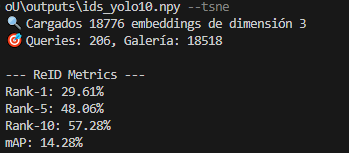
\includegraphics[width=0.8\textwidth]{image/metricas_reid_yolo10}
 		\caption{\textbf{Resultado ReID Yolov10}}
 		\label{fig:Resultado Yolov10 reid}
 	\end{figure}
 	
 	\begin{figure}[H]
 		\centering
 		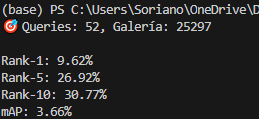
\includegraphics[width=0.8\textwidth]{image/metricas_reid_deepEIoU}
 		\caption{\textbf{Resultado ReID DeepEIoU con Osnet entrenado con el dataset de Sportmot}}
 		\label{fig:Resultado DeepEIoU con Osnet reid}
 	\end{figure}
 	
 	\subsection{Resultados de MOT comparando YOLOv10 y YOLOX}
	
	\begin{figure}[H]
		\centering
		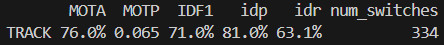
\includegraphics[width=0.8\textwidth]{image/metricas_mot_yolo10}
		\caption{\textbf{Resultado MOT Yolov10}}
		\label{fig:Resultado Yolov10 mot}
	\end{figure}
	
	\begin{figure}[H]
		\centering
		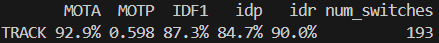
\includegraphics[width=0.8\textwidth]{image/metricas_mot_deepEIoU_osnet_sportmot}
		\caption{\textbf{Resultado MOT DeepEIoU con Osnet entrenado con el dataset de Sportmot}}
		\label{fig:Resultado DeepEIoU con Osnet mot sportmot}
	\end{figure}
	
	\begin{figure}[H]
		\centering
		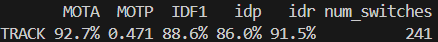
\includegraphics[width=0.8\textwidth]{image/metricas_mot_deepEIoU_osnet_soccernet}
		\caption{\textbf{Resultado MOT DeepEIoU con Osnet entrenado con el dataset de Soccernet}}
		\label{fig:Resultado DeepEIoU con Osnet mot soccernet}
	\end{figure}
	
	resnet50\_fc512
	
	\section{Dificultades encontradas}
	
	
	
	\section{Conclusiones}
	
	
	
	%%%%%%%%%%%%%%%%%%%%%%%%%%%%%%%%%%%%%%%%%%%%%%%%%%%%%%%%%%%%%%%%%%%%%%%%%%%
	\printbibliography
	
	
	%% Back Cover
	
\includepdf[noautoscale=true, width=\paperwidth]{backcover.pdf}
	
\end{document}